\documentclass[10pt,oneside]{memoir}
\usepackage{layouts}[2001/04/29]
\makeglossary
\makeindex

\def\mychapterstyle{default}
\def\mypagestyle{headings}
\def\revision{}

%%% need more space for ToC page numbers
\setpnumwidth{2.55em}
\setrmarg{3.55em}

%%% need more space for ToC section numbers
\cftsetindents{part}{0em}{3em}
\cftsetindents{chapter}{0em}{3em}
\cftsetindents{section}{3em}{3em}
\cftsetindents{subsection}{4.5em}{3.9em}
\cftsetindents{subsubsection}{8.4em}{4.8em}
\cftsetindents{paragraph}{10.7em}{5.7em}
\cftsetindents{subparagraph}{12.7em}{6.7em}

%%% need more space for LoF numbers
\cftsetindents{figure}{0em}{3.0em}

%%% and do the same for the LoT
\cftsetindents{table}{0em}{3.0em}

%%% set up the page layout
\settrimmedsize{\stockheight}{\stockwidth}{*}	% Use entire page
\settrims{0pt}{0pt}

\setlrmarginsandblock{1.5in}{1.5in}{*}
\setulmarginsandblock{1.5in}{1.5in}{*}

\setmarginnotes{17pt}{51pt}{\onelineskip}
\setheadfoot{\onelineskip}{2\onelineskip}
\setheaderspaces{*}{2\onelineskip}{*}
\checkandfixthelayout

\usepackage{fancyvrb}			% Allow \verbatim et al. in footnotes
\usepackage{graphicx}			% To include graphics in pdf's (jpg, gif, png, etc)
\usepackage{booktabs}			% Better tables
\usepackage{tabulary}			% Support longer table cells
\usepackage[utf8]{inputenc}		% For UTF-8 support
\usepackage[T1]{fontenc}		% Use T1 font encoding for accented characters
\usepackage{xcolor}				% Allow for color (annotations)

%\geometry{landscape}			% Activate for rotated page geometry

%\usepackage[parfill]{parskip}	% Activate to begin paragraphs with an empty
								% line rather than an indent


\def\myauthor{Author}			% In case these were not included in metadata
\def\mytitle{Title}
\def\mykeywords{}
\def\mybibliostyle{plain}
\def\bibliocommand{}

\VerbatimFootnotes
\def\affiliation{AGH University of Science and Technology}
\def\myauthor{Mateusz Łapsa-Malawski}
\date{2005}
\def\mydate{2005}
\def\email{ \href{mailto:mateusz@munhitsu.com}{mateusz@munhitsu.com}}
\def\format{complete}
\def\mytitle{Risk evaluation system for Specific Immunotherapy patients based on ANN and Genetic Algorithms}
\def\web{\href{http://munhitsu.com/}{http://munhitsu.com/}}


%
%	PDF Stuff
%

%\ifpdf							% Removed for XeLaTeX compatibility
%  \pdfoutput=1					% Removed for XeLaTeX compatibility
  \usepackage[
  	plainpages=false,
  	pdfpagelabels,
  	pdftitle={\mytitle},
  	pagebackref,
  	pdfauthor={\myauthor},
  	pdfkeywords={\mykeywords}
  	]{hyperref}
  \usepackage{memhfixc}
%\fi							% Removed for XeLaTeX compatibility


%
% Title Information
%


\ifx\latexauthor\undefined
\else
	\def\myauthor{\latexauthor}
\fi

\ifx\subtitle\undefined
\else
	\addtodef{\mytitle}{}{ \\ \subtitle}
\fi

\ifx\affiliation\undefined
\else
	\addtodef{\myauthor}{}{ \\ \affiliation}
\fi

\ifx\address\undefined
\else
	\addtodef{\myauthor}{}{ \\ \address}
\fi

\ifx\phone\undefined
\else
	\addtodef{\myauthor}{}{ \\ \phone}
\fi

\ifx\email\undefined
\else
	\addtodef{\myauthor}{}{ \\ \email}
\fi

\ifx\web\undefined
	\else
		\addtodef{\myauthor}{}{ \\ \web}
\fi

\title{\mytitle}
\author{\myauthor}

\begin{document}

\chapterstyle{\mychapterstyle}
\pagestyle{\mypagestyle}

%
%		Front Matter
%

\frontmatter


% Title Page

\maketitle
\clearpage

% Copyright Page
\vspace*{\fill}

\setlength{\parindent}{0pt}

\ifx\mycopyright\undefined
\else
	\textcopyright{} \mycopyright
\fi

\revision

\begin{center}
\framebox{ \parbox[t]{1.5in}{\centering Formatted for \LaTeX  \\ 
 by MultiMarkdown}}
\end{center}

\setlength{\parindent}{1em}
\clearpage

% Table of Contents
\tableofcontents
%\listoffigures			% activate to include a List of Figures
%\listoftables			% activate to include a List of Tables


%
% Main Content
%


% Layout settings
\setlength{\parindent}{1em}

\mainmatter
\part{Risk evaluation system for Specific Immunotherapy patients based on ANN and Genetic Algorithms}
\label{specificimmunotherapypatientsriskevaluationsystembasedonannandgeneticalgorithms}

AGH University of Science and Technology
Faculty of Electrical Engineering, Automatics, IT and Electronics
Computer Science
M.A. Thesis


Author: Mateusz Łapsa-Malawski
Supervisor: PhD, D.Eng Marek Valenta
Date: Kraków 2005


\part{Acknowledgements}
\label{acknowledgements}

\begin{itemize}


\item To prof. Marek Valenta, for his patience and helping in organizing this thesis;

\item To prof. Joanna Grabska-Chrząstowskiej, for advice on neural networks;

\item To dr. Ewa Cichocka-Jarosz, for introducing me to the world of immunology, sharing data and constant advising
\end{itemize}

\begin{quotation}
``Every hospital should have a plaque in the physicians' and students' entrance: There are some patients whom we cannot help; there are none we cannot harm.''
Arthur L. Bloomfield
\end{quotation}

\part{Introduction}
\label{introduction}

The increase in data processing capabilities of modern computers and the development of analytical tools allows to create more and more sophisticated computing systems. In the beginning, they were just assisting people in organizational and bookkeeping tasks, cataloguing the data and therefore decreasing access time. Now, while still supporting users, they attempt to play the role of domain experts.
It is estimated that 10-20\% of population suffers from allergy-related conditions. That number is even higher among children - 20-30\%. Symptoms can range from almost undetectable to excessive continuous swelling resulting in serious changes in the patients' organisms.  After establishing which allergen is responsible, the attempts are made to alleviate the symptoms and, at the same time, to remove the allergen from the patients surroundings. Unfortunately this is not always possible, for example in case of the grass pollen allergy.
The thesis is an attempt of a secondary analysis of data collected during clinical tests on specific immunotherapy (SIT), conducted by Dr. Ewa Cichocka-Jarosz ~\cite{Cichocka-Jarosz:1997}. SIT is a long-term therapy, which aims at decreasing the discomfort of allergy symptoms. Regular visits at a clinic are required, increasing the costs and causing further inconvenience for the patients.
The research at the Department of Biostatistics and Medical Informatics at Colllegium Medicum of the Jagiellonian University comprised of a complete standard statistical analysis of the data using the SAS software suite. Tests conducted included, among others:


\begin{itemize}


\item Repeated variance analysis tests (ANOVA), with additional verification of the means' differences using the Duncan test for normal distribution variables

\item Kruskall-Wallis test for remaining variables ~\cite{Cichocka-Jarosz:1997}
\end{itemize}

\begin{quotation}
The aim of the thesis is to develop, based on the knowledge extracted from existing data, a decision support system, assisting doctors in prescribing an appropriate  therapy path to the patients.
\end{quotation}

The system should assess risks and adequacy of the prescribed treatment.


Specific immunotherapy is a new method of allergy treatment, therefore the number of publications on patients' responsiveness to therapy is small. The author is not aware of any computer system related to SIT.
The data analyses performed for the purposes of this thesis were conducted utilizing artificial neural networks and genetic algorithms. Initial trial of predicting the patients' chances for deterioration after beginning therapy was not satisfactory. Due to limited amount of learning data system was not able to precisely describe the level of deterioration of patients' condition. It could, however, predict tendencies. Rate of success for predicting the increase of symptoms during therapy was 72\%. The objective of building a decision support system has been met.
Additionally, a system allowing for heuristic selection of optimal neural network and training it, was tested.


An introduction to immunotherapy can be found in Chapter 2 (\autoref{chapter2}). Being different in scope than the rest of the thesis, this chapter also provides some information on the functions of the immune system. The issues relating to neural networks are outlined in Chapter 3 (\autoref{chapter3}). Emphasis was put on multilayered networks, as they were later used when predicting the therapy outcomes. A discussion on genetic algorithms used to select the neural network architecture is featured in Chapter 4 (\autoref{chapter4}). Chapter 5 (\autoref{chapter5}) contains information on the initial data preparation and analysis. The analysis was based on Statistica Neural Networks 6 software suite and the JIM system, which was created by the author. JIM made possible the initial data preparation and, at the later analytic stage, the heuristic selection of the network. Chapter 6 (\autoref{chapter6}) is focused on the JIM system. Discussed are its capabilities and the choice of technologies utilized. Chapter 7 (\autoref{chapter7}) discusses the results obtained and the technologies employed.
The thesis is concluded with the bibliographical review, Appendix A (\autoref{appendixa}) (specifications of the JIM computer system created) and the Appendix B (\autoref{appendixb}) (listing the contents of the attached CD).


\part{Immunology}
\label{chapter2}

Despite the fact that the allergology is a relatively new field, its roots can be traced to the beginning of the XIX century. In 1819, John Bostock described a ``periodical affection of the eyes and chest'', now known as pollenosis or, more commonly, hay fever. ``It is commonly thus assumed, that it (the ailment) is caused by dust from the fresh hay'' (quotation from 1.). After trying to look for this condition among the Englishmen, he could only diagnose 28 cases. Obviously it was a marginal problem. Not until the middle of the XIX century its connection to pollen was observed and proved by Charles Blackley. His experiments with using a sticky microscope slide tied to a kite allowed him to demonstrate the presence of pollen at 500m above ground level. That meant it could be spread with the wind over large distances. Blackley was able to thus explain why he himself suffered from hay fever living in Manchester, without any direct exposure to plants producing allergenic pollen. Only in 1905 two pediatricians, Clemens von Pirquet and Bela Shick, proposed the term ``allergy'' to describe a varied responsiveness of human organism. After that, society began talking about innate predisposition to allergy in some organisms.
An interesting case has been observed in 1919. Dr. Maximilian Ramirez treated a patient who apparently contracted asthma through a blood transfusion. Before then, the patient had been frequently around horses with no adverse effects. Then, after the transfusion, he had the first fit of the disease while enjoying a horse ride. It later turned out that the blood donor was an asthmatic, whose skin tests came out positive for horse hair. That case suggested there might exist a substance in blood that is responsible for allergies. That hypothesis had been developed by Prausnitz and Kustne, who proposed an existence of a blood agent, later called ``reagin''.
For a long time the immunology was not taken seriously, which resulted from, among others, a lack of precise research methods. A breakthrough was achieved thanks to the work of two separate teams: Bennich and Johanson's and the Ishizakawas' husband-wife team. They discovered a previously unknown immunoglobulin: immunoglobulin E (IgE) that encompasses also reagin antibodies. The teams shared their findings in 1968 and were awarded a Nobel Prize the next year. Allergology became a subfield of the clinical immunology.


\chapter{The immune system}
\label{theimmunesystem}

The human organism is constantly threatened by ``intruders''. Defending against them and their removal is the responsibility of innate (nonspecific) and adaptive (specific) immune systems. External mechanisms of resistance include defensive barriers of epidermis and mucosal membrane.
The surface of the epidermis is acidic, which prevents the growth of bacterial populations. Additionally, it is covered by suet, the sebaceous gland secretion, which is comprised of bacteria-killing unsaturated fatty acids. An important defensive mechanism of the epidermis is its constant shedding.
Mucous membranes, potentially easier to penetrate for allergens, are covered with mucus, which is strongly antiseptic (lysozymes, interferon, and defensins). Additional antiseptic barrier in digestive and excretory systems is provided by the acidity of urine and gastric acid ~\cite{Resmedica:UkladImmunologiczny}.
After the antigen penetrates the skin or mucous membrane, cellular-level innate immune mechanisms are activated and deliver a quick defensive response. These are the circulatory system cells, tasked with engulfing and digesting pathogens (macrophages, neutrophil granulocytes). Innate immune system also includes a special group of lymphocytes - natural killers (NK), whose main role is to destroy cancerous or virus-infected cells.
Adaptive immunity systems, phylogenetically younger, target specific antigens and require more time to fully activate. Once started, they will deliver a timely, precise and effective protection on every future occasion, thanks to their immunological memory. Two populations of lymphocytes provide fundamental mechanism of the adaptive immune system: B cells, producing antibodies (immunoglobine M, immunoglobine E) and T cells, capable of  recognizing a specific antigen using their receptors. Two main types of T cells are CD4+ (T helper, Th) and CD8+ (cytotoxic T cell, Tc). Th cells of Th1 phenotype induce a specific inflammatory reaction, while the Th2 phenotype Th cells reduce inflammations, while stimulating IgE-dependent allergic reactions.
APC (Antigen Presenting Cells) are the cells allowing the T cells to recognize the intruding antigens. Depending on the antigen penetration route, the role of the APC can be performed by skin cells (Langerhans cells), monocytes of the circulating blood, tissue macrophages, or dendritic cells of the nervous system. After intercepting the antigen, they travel through the lymphatic vessels to the lymph nodes, where they present it to the T cells and stimulate the T cells specific response. They display the external molecule on their surface, together with the tissue compatibility antigens. For the T cells to activate, an interaction between particular receptors on surfaces of T cells and APCs is required.
Activated T cells produce particular cytokines. They are a signal for the B cells, which transform into plasmatic cells and synthesize a special type of antibodies. Most common is the immunoglobulin G fraction, comprising of 4 subclasses: $ I{gG}_{1}$, $ I{gG}_{2}$, $ I{gG}_{3}$, and $ I{gG}_{4}$. Defenses of the mucous membranes are founded upon the so called secretory IgA. Immunoglobulin M takes part in processes connected with phagocytosis and cells' digestive functions. Immunoglobulin E is essential for the anaphylactic reactions. The functions of Immunoglobulin D are not well known.


\chapter{IgE-dependent allergy}
\label{ige-dependentallergy}

This disorder is an innate oversensitivity of the organism to given external agent existing in low concentrations. The most common allergens are substances present in air, called aeroallergens (dust mites, pollen, molds, animal hair and epidermis). Allergies to foods (grains, proteins of egg whites and yolks) are rarer and usually affect younger children. Patients suffering from IgE-dependent allergies typically have more Th2 phenotype T cells. Cytokines, produced by those cells, stimulate synthesizing of the allergen-specific IgE antibodies tied on the surface of the mast cells and also activate eosinophil granulocytes, which results in a chronic inflammatory reaction. When the allergen concentration reaches a defined level, mast cells activate (degranulate), releasing the inflammation mediators. Those include, among others: histamine (determining clinical symptoms like fits of sneezing, teary eyes, dyspnea or nettle-rash), cytokines (stimulating other cells into allergic reaction) or metabolite of the arachidonic acid (sustaining the inflammation).


\chapter{The increase in the number of allergies}
\label{theincreaseinthenumberofallergies}

Recently, there is a dynamic increase in the number of those affected by allergies (Grevers, Rocken, 2002). Epidemiological surveys proved that 25-30\% of population in developed countries suffer from allergic ailments. Allergies have been the subject of many epidemiological and genetical research projects, whether clinical, experimental or environmental.
There are international research project carried: IUATLD (asthma among adults), ISAAC (International Study of Asthma and Allergy in Childhood). It has been established that, besides genetic factors, child's environment (concentration of the allergens, pollution) and the types of food introduced in the diet during the first year of life are essential in the development of allergies.


\chapter{Allergen - specific Immunotherapy}
\label{allergen-specificimmunotherapy}

Specific immunotherapy is the only currently known method of etiologic treatment of the pathomechanism of IgE-dependent allergies. The method has a proven positive effect on patients suffering from allergic rhinitis and conjunctivitis, as well as milder forms of asthma. For those allergic to hymenoptera venom (bees, wasps and hornets) it is a risk factor-determined treatment. The treatment consists of subcutaneous administrations of increasing dosages of purified allergen. The most common ones are pollen (trees, grass, rye, weeds) and dust mites. The objective of the therapy is to develop a tolerance of the immune system. Due to a degree of inertia of the process, the treatment usually lasts about 3 to 5 years. When treating patients allergic to pollen, the desensitization is performed a couple of weeks before the given plant's pollen season. In case of grass allergy, the treatment takes place between February and April. Those allergic to dust mites require a year-round therapy. Strict qualification criteria include confirmation of the IgE-dependency of the ailment (positive skin tests, high level of IgE typical for a given allergen), together with typical clinical symptoms observed. Even assuming correct qualification, 10\% of treated do not show any improvement ~\cite{Alergologia:1998}. Because of the length of treatment, costs for the patients and trauma (injections), it is important to improve the precision of the qualifying criteria.
During the treatment it is common to increase the level of medicating the patient. Moreover, it is actually possible to further sensitize the patient, that is to increase the allergic reaction, or even develop an allergy to different allergen ~\cite{Cichocka-Jarosz:1997}.


The underlying mechanisms of specific immunotherapy are not well known. Observed effects include:


\begin{enumerate}


\item Changing of T cells phenotypes:

\item Prominent increase of the number of regulatory T cells (Tr)

\item Increase of the number of Th1 T cells

\item Decrease in the number of Th2 lymphocytes, which mediate the IgE-dependent reactions.

\item Increased apoptosis (dying of cells) of the Th2 lymphocytes

\item An increase  of the concentration level of the cytokines typical for Th1 cells (interferon $\gamma $, interleukin 2)

\item A decrease in the concentration level of Th2 typical cytokines (interleukin 4, interleukin 5, GM-CSF)

\item Stimulating of the blocking antibodies production (IgG class)
\end{enumerate}

Regardless of changes in immunological parameters, the most important criterion of improvement is the patients' subjective perception of a decrease of discomfort and limiting the amount of medications administered.


\part{Introduction to artificial neural networks}
\label{chapter3}

Artificial neural networks are algorithmic structures modeled after the biological structure of the brain. They are an effective tool for predicting, classifying and approximating of data. They are also a way of understanding the essence of the human mind and its self-awareness. Cognitive science is a field devoted to investigating the mind in a broader scope compared to psychiatry, psychology, neurology and philosophy ~\cite{Duch:2004:NaukiKognitywne}.
The following chapter discusses the problem of simulating the mind and its structure at the level of singular cells.


\chapter{Structure of the brain}
\label{structureofthebrain}

The brain is a wrinkled structure, in which two cerebral hemispheres, medulla and brainstem can be distinguished ~\cite{Jura:Krzanowska:1992}. The cells that the brain matter is comprised of are nerve cells and glial cells. There are 10 glial cells for each nerve cell.
Cross section of the brain reveals grey and white matters. White matter, found inside the brain, is comprised of nerve fibers and glial cells. Grey matter (cerebral cortex), constituting the external layer of the brain, is comprised of nerve cells and also glial cells. White matter transmits data, grey matter processes it.


\section{Nerve cells}
\label{nervecells}

The basic building block of the brain is the neuron. A human brain is comprised of about 100 billion nerve cells ($ {10}^{11}$) ~\cite{Greenfield:1999}, and about 100 trilliard ($ {10}^{15}$) connections between them ~\cite{Veggeberg:1996}.


Following are the known elements of a neuron:


\begin{itemize}


\item Cell body (soma)

\item Nucleus

\item Axon

\item Dendrites

\item Synapses
\end{itemize}

Nerve cells are diploidic and adapted to transmitting and modifying electrical impulses. They have nuclei and typical organelle suspended in cytoplasm. They do not, however, possess centrioles responsible for cell replication. Axons are long, fibrous projections of neurons, which transmit output signals to other cells. Axons are shielded by myelin, which acts as an insulator. Synapses are attached to axons' ends. They are points of contact between nerve cells and other electro active cells (nerve or muscle cells). Synapses carry impulses with the help of synaptic mediators or as an electrical impulse ~\cite{Jura:Krzanowska:1992}.
Dendrites are extensions of nerve cells which receive signals from other neurons. Their structure is usually tree-shaped, but there exist cells with dendrites similar to axons. Depending on type, a dendrite is capable of suppressing or amplifying signals. Signals are temporarily stored in the nucleus. When their number is higher than the threshold capacity of a given cell, an output signal is generated. Neurons are capable of transmitting up to 500 signals per second.


\section{Glial cells}
\label{glialcells}

General types of glial cells include astrocytes, oligodendrocytes, Schwann cells and microglia. It is believed that glial cells support nerve cells.
Their known function is to maintain a proper composition of the fluid filling the intracellular spaces in the nerve tissue. Too high concentration of K+ ions, excreted by neurons, could lead to blocking of the cell. Astrocytes have a known function of absorbing those ions. Besides that, the glial cells nutrify neurons. They also play an important part during the development of the organism. Then, they create a type of protein paths, which lead neural extensions to other cells ~\cite{Szarski:1976}, e.g.\ nerve or muscle cells. Oligodendrocytes create a myelin sheath around neural extensions, which speeds up the transmission of impulses. Schwann cells are part of axons' myelin sheaths.
In recent years, research has shown the role of glutamate in the functioning of the nervous system. There is a hypothesis that through the emission of glutamate, the astrocytes can communicate with neurons using neurotransmitters and modify their functions. The frequency of their emission is 5Hz. If we keep in mind that astrocytes have branched-out structure, it becomes apparent that a single cell can interact with around 140 thousand synapses \cite{Bezzi:Gundersen:2004}.


\chapter{Brain simulation}
\label{brainsimulation}

Full simulation of the brain is based on the following assumptions:


\begin{itemize}


\item Complete mechanisms of a nerve cell activity is known

\item Mechanisms of mind development and external connections are known

\item It is possible to simulate a complete network

\item Simulated network will be fed data similar to that received by a human brain during a lifespan of an individual
\end{itemize}

A network of connected neurons is a known, simplified model of a brain, if we assume that one modulation of an input signal is an ``x'' of floating-point computations
Furthermore, calculating the output value is ``y'' floating-point operations. Computing power needed for simulating neurons equals 500 actions per second * ($ x\cdot {10}^{15}$ inter-cell connections + $ y\cdot {10}^{11}$ cells). If we assume that $ x=y=1$, then a machine capable of $ 500\cdot ({10}^{15}+{10}^{11})\approx 5$ PFlops is needed. For comparison, the computing power of the currently fastest computing cluster, BlueGene/L, equals 135 TFlops. An installation of 350 TFlops capable BlueGene/L is scheduled for 2005 ~\cite{IBM:2005:Bluegene}.
For the estimations we've assumed that the cell model is simple, so that a dendrite modulates a signal in one operation, and a cell processes it also as a single operation. This assumption is appropriate with the basic model of perceptron ~\cite{Camargo:1990}. Note that if one want to model the whole brain, and not just some characteristics of its part, than a complete model of possibly higher complexity would be required.


\chapter{Nerve cell simulation}
\label{nervecellsimulation}

Research on neuron structure resulted in a general behaviour model of this type of cell. Main guidelines are contained in the perceptron model ~\cite{Tadeusiewicz:1993}. Its structure consists of:


\begin{figure}
\begin{center}
\resizebox{1\linewidth}{!}{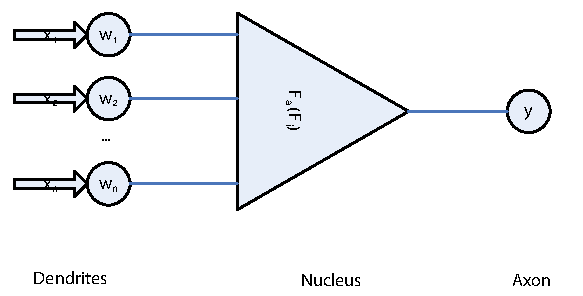
\includegraphics{fig1.pdf}}
\end{center}
\label{figure1}
\end{figure}

Figure 1 Nerve cell model


\begin{itemize}


\item Dendrites
Data inputs. They initially process a single input signal ($ {x}_{i}$). That means amplifying or suppressing it, depending on its weight ($ {w}_{i}$).

\item Nucleus
Computational center. Adds modulated data coming in from the dendrites and then transmits the signal to an axon depending on the defined activation function ($ {F}_{a}$). J.Mulawka defines an auxiliary function $ {F}_{i}$~\cite{Mulawka:1996}, which initially processes input sum: $ \sum _{i=0}^{n}{X}_{i}{W}_{i}$

\item Axon
Singular data output. It connects to the dendrites of other cells.
\end{itemize}

\begin{equation}
y={F}_{a}\left({F}_{i}\left(\sum _{i=0}^{n}{X}_{i}{W}_{i}\right)\right)
\end{equation}


Following variants are known:


\textbf{Linear model}


Activation and initial processing functions are expressed as y=x, so the neuron is:


\begin{equation}
y=\sum _{i=0}^{n}{X}_{i}{W}_{i}
\end{equation}


Function value graph for two equivalent inputs:


\begin{figure}
\begin{center}
\resizebox{1\linewidth}{!}{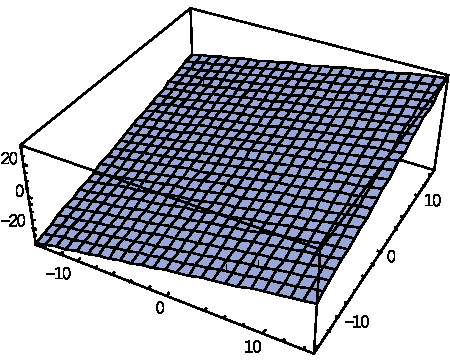
\includegraphics{fig2.pdf}}
\end{center}
\label{figure2}
\end{figure}

Figure 2 Linear model


\textbf{Nonlinear discrete model}


Activation function is defined as:


\begin{equation}
{F}_{a}\left(x\right)=\{\begin{array}{ll}1& x>\Theta \\ 0& x\le \Theta \end{array}
\end{equation}


Initial processing function as:


\begin{equation}
{F}_{i}\left(x\right)=x
\end{equation}


Where $ \Theta $ is defined as neuron's threshold value. It is known as TLU (Threshold Logic Unit). The graph of the activation function for two equivalent inputs (threshold: $ \Theta =1$):


\begin{figure}
\begin{center}
\resizebox{1\linewidth}{!}{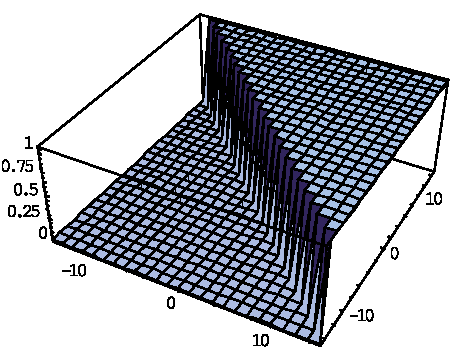
\includegraphics{fig3.pdf}}
\end{center}
\label{figure3}
\end{figure}

Figure 3 Discrete model


\textbf{Nonlinear sigmoidal model}


Activation function is expressed as:


\begin{equation}
{F}_{a}\left(x\right)=\frac{1}{1+{e}^{\Theta -x}}
\end{equation}


Initial processing function as:


\begin{equation}
{F}_{i}\left(x\right)=x
\end{equation}


Where $ \Theta $ is the neuron's threshold value.
Graph of the activation function for two equivalent inputs (threshold: $ \Theta =1$):


\begin{figure}
\begin{center}
\resizebox{1\linewidth}{!}{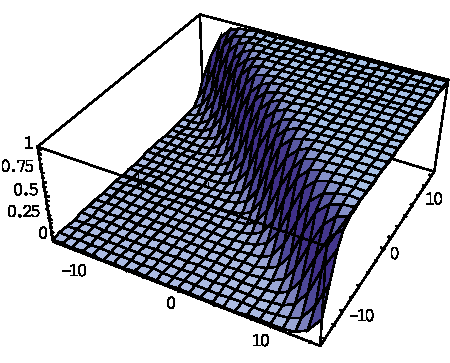
\includegraphics{fig4.pdf}}
\end{center}
\label{figure4}
\end{figure}

Figure 4 Sigmoidal model


After the critical input signal energy of a given cell is exceeded, the cell emits an impulse. The closest model of that behaviour was the TLU model. Regrettably, because the derivative is not continuous, it is not easy to train. However, the sigmoidal model is very promising, because it is structurally similar to the discrete model and there exists a simple derivative for it


\begin{equation}
\frac{d{F}_{a}}{x}={F}_{a}\left(x\right)(1-{F}_{a}\left(x\right))
\end{equation}


Additionally, the slope curvature, used as a component, has proven to be very usable for modeling of complex functions.


\section{Geometric interpretation}
\label{geometricinterpretation}

When we look at a neuron with a single input, we can see that functions as a classifier. Depending on the activation function employed its response will be as follows.


For discrete nonlinear:


\begin{figure}
\begin{center}
\resizebox{1\linewidth}{!}{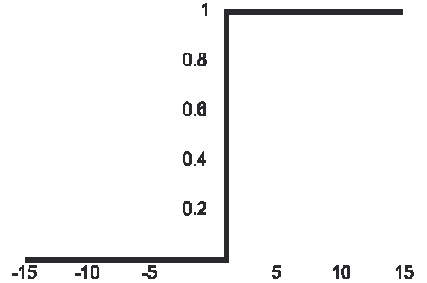
\includegraphics{fig5.pdf}}
\end{center}
\label{figure5}
\end{figure}

Figure 5 Discrete activation function


For sigmoidal:


\begin{figure}
\begin{center}
\resizebox{1\linewidth}{!}{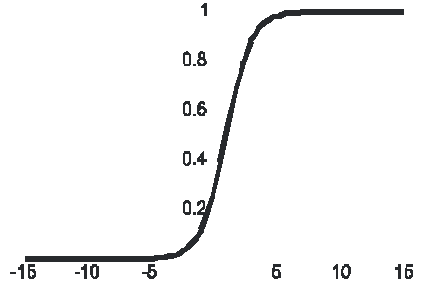
\includegraphics{fig6.pdf}}
\end{center}
\label{figure6}
\end{figure}

Figure 6 Sigmoidal activation function


For a single value we have one-dimensional area, divided in two parts by the threshold\footnote{Two sets of points A and B on n-dimensional input space are linearly separatable if there exists n+1 of  $ {w}_{1},...,{w}_{n+1}$, such that every point $ x\in A$ satisfies $ \sum _{i=1}^{n}\left({W}_{i}{X}_{i}\right)\ge {W}_{n+1}$ , and every $ y\in B$ satisfies $ \sum _{i=1}^{n}\left({W}_{i}{Y}_{i}\right)\ge {W}_{n+1}$}. If we increase the number of inputs to 2 we get the situation depicted on Figure 4 (\autoref{figure4}). 3-dimensional space will be divided by a plane. This interpretation can be extended with further dimensions \cite{Camaro:1990}. In effect, a neuron functions as a linear classifier, or, put differently, a ``linear separator'' ~\cite{Podolak:2003:Perceptron}.
Let ``X'' be the inputs vector, and ``W'' the weights vector. Then the sum of products of inputs and their weights is a dot product of two vectors:


\begin{equation}
X\star W=\sum _{i=0}^{n}\left({X}_{i}{W}_{i}\right)
\end{equation}


This product is compared to threshold value $\Theta $. So the threshold function is:


\begin{equation}
\Theta =\sum _{i=0}^{n}\left({X}_{i}{W}_{i}\right)
\end{equation}


Alternatively:


\begin{equation}
\sum _{i=0}^{n}\left({X}_{i}{W}_{i}\right)-1\cdot \Theta =0
\end{equation}


Increasing the number of inputs by ``-1'' allows for interpreting the threshold value as a weight:


\begin{equation}
\sum _{i=0}^{n+1}\left({X}_{i}{W}_{i}\right)=0
\end{equation}


Going further: neuron's value is a scalar product of the extended input vector and the extended weights vector compared to 0. Alternatively:


\begin{equation}
X\star W=\left|\left|X\right|\right|\times \left|\left|W\right|\right|cos\alpha 
\end{equation}


Where $ \alpha $ is the angle of the vectors. From the neuron's perspective, it being a classifier, the only important factor is whether the value higher or equal than 0, or lower than 0. $ cos\left(\alpha \right)$ gives the answer to this question.
The value of a neuron, then, depends on the angle between the weight vector and inputs vector.


\begin{equation}
\alpha \in <0,\pi ):
\end{equation}


\begin{equation}
\alpha \le \frac{\pi }{2}\to 1
\end{equation}


\begin{equation}
\alpha >\frac{\pi }{2}\to 0
\end{equation}


\section{The Delta rule}
\label{thedeltarule}

Delta rule, developed by Widrow and Hoff ~\cite{Widrow:Hoff:1960}, known also as the Least Mean Square (LMS) method, is the most common algorithm for training neurons.


The starting point is the definition of an error. Squared difference between the output and the expected output values is used. For a single neuron:


\begin{equation}
{E}_{p}=\frac{1}{2}{(t-y)}^{2}
\end{equation}


Increasing the number of neurons:


\begin{equation}
E=\sum _{p}{E}_{p}=\sum _{p}\left(\frac{1}{2}{(t-y)}^{2}\right)
\end{equation}


The method consists of a gradual modification of weights, so that the error function's minimum can be found:


\begin{equation}
{w}_{i}^{j+1}={w}_{i}^{j}+\Delta {w}_{i}j
\end{equation}


Level of change depends on the error level, hence the gradient descent method.


\begin{equation}
\Delta {w}_{i}=-\eta \frac{\partial {E}_{p}}{\partial {w}_{i}}
\end{equation}


$-\eta $ is the learning rate. Expanding the derivative we obtain:


\begin{equation}
\frac{\partial {E}_{p}}{\partial {w}_{i}}=\frac{\partial {E}_{p}}{\partial y}\cdot \frac{\partial y}{\partial {w}_{i}}=\frac{\partial {E}_{p}}{\partial y}\cdot \frac{\partial y}{\partial e}\cdot \frac{\partial e}{\partial {w}_{i}}
\end{equation}


Calculating:


\begin{equation}
\frac{\partial {E}_{p}}{\partial y}=-(t-y)
\end{equation}


\begin{equation}
\frac{\partial e}{\partial {w}_{i}}={x}_{i}
\end{equation}


A sigmoid is used as the activation function, thanks to its derivative and a simple way to calculate the ``e'' argument:


\begin{equation}
y\left(x\right)=\frac{1}{1+{x}^{-\beta e}}
\end{equation}


\begin{equation}
\frac{\partial y}{\partial e}=y(1-y)
\end{equation}


Summing up:


\begin{equation}
\Delta {w}_{i}=-\eta \frac{\partial {E}_{p}}{\partial y}\cdot \frac{\partial y}{\partial e}\cdot {x}_{i}
\end{equation}


\begin{equation}
\Delta {w}_{i}=\eta (t-y)\frac{\partial y}{\partial e}\cdot {x}_{i}=\eta (t-y)(1-y){x}_{i}y
\end{equation}


We obtained a change of the weight as functions of: desired value, network response and current neuron's input.


\chapter{Glial cell simulation}
\label{glialcellsimulation}

Simulating glial cells is not a well explored area and is certainly worth of further investigation. An interesting addition to the SSN model would be to expand it with slower cells with much higher number of connections, which would simulate the glial cells.


\chapter{Types of networks}
\label{typesofnetworks}

Despite its severe limitations (or maybe thanks to them!), the perceptron turned out to be worthy of further examination. It has many interesting features: linearity, intriguing assumption of convergence, paradigmatic simplicity as the method of parallel computing. There are no reasons to think that any of those qualities will translate to its multi-layer form. However, we still think that serious research is needed to accept (or dismiss) our thesis that expanding to multilayer systems is futile, ~\cite{Minsky:Papert:1969}


\section{Multilayer perceptron}
\label{multilayerperceptron}

Multi-layered model is the typical example of the topology. A single layer is composed of independent neurons and acts as a filter. Neurons of subsequent layers are connected on an ``each to each'' principle. Every layer can contain a different number of neurons. In the input layer, a single neuron is associated with every single piece of data (input stream, picture point). Frequently, input data is preliminarily processed. Symbolic data are assigned either a numeric value, or a separate logic input for individual symbols. Normalizing of numeric data is recommended. Subsequent layers are referred to as ``hidden layers''. Depending on the complexity of a problem, two or three of those are used. Employing a larger number significantly increases the length of network's training without improving its quality. Depending on the number of neurons in hidden layers and the length of learning, the network can either generalize or learn the input data set. The last layer is the output layer. In classifying networks, it consists of as many outputs as the number of expected classes.


\begin{figure}
\begin{center}
\resizebox{1\linewidth}{!}{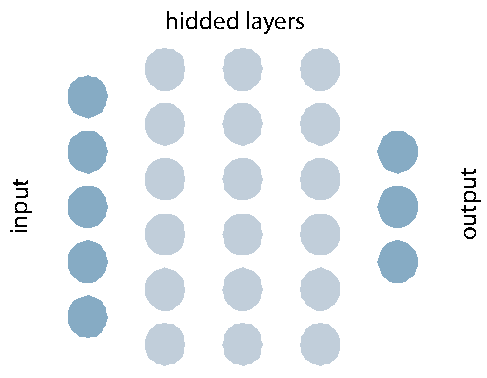
\includegraphics{fig7.pdf}}
\end{center}
\label{figure7}
\end{figure}

Figure 7 Multilayer perceptron


\section{Backpropagation}
\label{backpropagation}

Training of a network consists of simultaneously training individual neurons employing the delta method. Training of the output layer is relatively simple. For each of its neurons, we know the expected output, and the current input and output (see 5.28).
To train the neurons of hidden layers, we need a definition of an error. We know the global output layer error.


\begin{equation}
E=\sum _{p}{E}_{p}=\sum _{p}\frac{1}{2}{(t-y)}^{2}
\end{equation}


Delta rule is still valid, however according to it, the error will be a weighted sum of subsequent layer errors. The layer is indicated in the upper index. Therefore:


\begin{equation}
\Delta {w}_{i}^{n}=-\eta \frac{\partial {E}_{p}^{n}}{\partial {w}_{i}^{n}}
\end{equation}


\begin{equation}
\Delta {w}_{i}^{n}=-\eta \frac{\partial {E}_{p}^{n}}{\partial {y}^{n}}\cdot \frac{\partial {y}^{n}}{\partial e}{x}_{i}
\end{equation}


Simplifying:


\begin{equation}
\Delta {w}_{i}^{n}=-\eta {\delta }^{n}{x}_{i}
\end{equation}


\begin{equation}
{\delta }^{n}=\frac{\partial {y}^{n}}{\partial e}\sum \left({\delta }^{m}{w}_{n}^{m}\right)
\end{equation}


Depending on the learning rate $ \eta $ the network can quickly find local minimum. Therefore, additional algorithms are often employed, to manipulate $ \eta $ so that the result is as close to the minimum as possible


\section{Conjugate Gradient Algorithm}
\label{conjugategradientalgorithm}

Conjugate gradient algorithm is a variation of the backpropagation algorithm. It cumulatively modifies the weights at the end of every training cycle, and not (like the backpropagation model does), after the presentation of every element of the training set.


\section{Other algorithms}
\label{otheralgorithms}

Completely different approach to training a network using a teacher is possible. In genetic algorithm methods, the network undergoes subsequent mutations. The algorithm is interesting, but not very efficient.


\section{Hopfield network as an example of a recurrent network}
\label{hopfieldnetworkasanexampleofarecurrentnetwork}

\begin{figure}
\begin{center}
\resizebox{1\linewidth}{!}{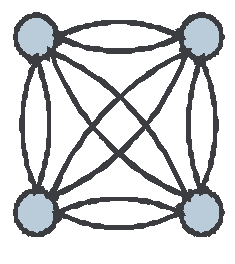
\includegraphics{fig8.pdf}}
\end{center}
\label{figure8}
\end{figure}

Figure 8 Recurrent network


Hopfield network is a type of associative memory. It is comprised of neurons connected to every other one, except themselves. Comparing it to the multilayer model, it is a looped single layered network, in which the neurons' connections with themselves are removed. Every neuron is both the input and the output. Network completes its task if after two iterations the output does not change, which means that the network gives out a stable output. It is used for identifying partially damaged pictures.


\section{Probabilistic neural networks}
\label{probabilisticneuralnetworks}

Bayes' theorem:


\begin{equation}
P\left(T|X\right)=\frac{P\left(T\right)P\left(X|T\right)}{P}\left(X\right)
\end{equation}


Probabilistic Neural Networks (PNN) are comprised of four layers:


\begin{itemize}


\item Input

\item Patterns

\item Summation

\item Output
\end{itemize}

In contrast with the models presented above, in PNN every node of the training set is associated to a separate neuron of the second layer.
Data classification is a typical application of PNN, since the output given by the network is a probability that the verified data belongs to a class. Training of these networks is quick, thanks to Bayes' theorem on dependent probability, but they are also very sensitive to the quality of data. The training set should be representative and quantitatively larger than the single element of the set (number of parameters specifying the element).


\part{Introduction to genetic algorithms}
\label{chapter4}

Genetic algorithms are an attempt to model the evolution of living organisms by using algorithms.
Every organisms grows according to the plan preserved in DNA, or RNA in case of simpler forms of life. Population of a given species is genetically varied. Thanks to that, it can survive sudden changes of the environment. Population members unfit for the new conditions die out, while the ones with needed characteristics (previously obsolete) now thrive and quickly rebuild the population. Now their genes appear more frequently within the population. Evolution takes place constantly, and organisms adapt to current environment, striving to dominate their ecospheres.
When creating a new organism, nature rarely uses cloning. Combining the genotypes of two specimens is more frequent. Before the zygote is created, the spermatozoon and the ovum undergo slight mutations. Eventually, a new organism appears. Before leaving the mother's body it undergoes a series of tests, to check whether it is worth of further ``investments''. Hence the frequent miscarriages among mammals. Amphibians employ a different strategy - single insemination results in numerous offspring, of which only few survive. The more adapted an organism is to its current environment, the better his chances of passing on its genes.


Genetic algorithms were developed by taking inspiration from these processes. They are heuristic algorithms, ideal for optimization of nontrivial functions.


\chapter{Mechanism}
\label{mechanism}

A problem is atomized by dissecting it into genes. They are often the parameters of the function being optimized. Usually, it is assumed that all specimens have one chromosome of the same length. Each gene describes a different parameter of a solution. A fitness function is created for every gene, describing how good the solution is.


The better the solution, the higher chance it has of producing offspring. Following methods of selection are used:


\begin{itemize}


\item Roulette method
Simple algorithm assigning each specimen a sector of a roulette wheel. The area of each fragment is directly proportional to the value of the fitness function

\item Tournament selection
The population is divided in two- or three member teams. One member of each team is selected to be transferred into parent pool of the next population. The selection of the transferred member can be either deterministic or nondeterministic (a variant of the deterministic method with the probability =1)

\item Rank selection
Members of the population are sorted according to their fitness function, in order to establish a ranking. Frequency of appearing in the parent pool of a next generation is a function of ranking and not the fitness.

\item Deterministic method
Divides the fitness function into integer and fractional parts. Integer part determines the member's frequency of appearing in the parent pool. This pool also includes members with biggest fractional parts.
\end{itemize}

The way of passing the genes to offspring is defined by the operators.
Commonly used are:


\begin{itemize}


\item Mutation operator
Operates on a single chromosome, creating a new chromosome with a randomly altered gene

\item Crossover operator
Operates on two chromosomes, creating a new one using randomly combined genes of parents. Its variants include:

\item One-point crossover
Single crossover point

\item Two-point crossover
Two crossover points

\item Multipoint crossover
Generalization of the previous two methods

\item Uniform crossover
A randomly selected pattern determines the choice of the gene's parent

\item Inversion operator
Operates on a single chromosome, inverting its selected fragment. Rarely used in genetic algorithms, although frequent among living organisms.
\end{itemize}

\part{Problem analysis}
\label{chapter5}

\chapter{Input data characteristics}
\label{inputdatacharacteristics}

A database containing records of 73 people was analyzed. That number included 53 patients and 16 healthy persons. Among patients, 31 were undergoing desensitization and 26 were treated conservatively.
Structure of the database is a two-dimensional matrix with 435 columns. A complete therapy history is coded in one row. Data gathered in fields include: age, patient's ID number, sex, medical history, medication taken, etc. This data was completely anonymous. The research was conducted in the Pulmonology Ward of the Polish-American Institute of Pediatry at the Collegium Medicum UJ ~\cite{Cichocka-Jarosz:1997}.
Data gathered is partially incomplete. The methodology of filling those gaps is presented further.


After the analysis of parameters used to describe cases and their timelines, parameters were grouped in the following way:


\begin{itemize}


\item Interview(wywiad)
mainly initial patient interviews - 14 parameters

\item Spring check-up (badania wiosenne)
Medical examination performed during spring - 54 parameters, grouped as follows:

\item w1
first year - before the beginning of treatment

\item w2{\ldots}w7
during following years of treatment

\item wk
during last year of treatment, depending on the length of treatment this data is copied from the w7 or w6 group




\item tests (testy)
additional set of tests, the so called specific allergen immunological system reactivity tests
14 parameters




\item testy\_1
done before the beginning of treatment

\item testy\_2
done during treatment

\item testy\_3
done in the final phase of the treatment

\item other
containing remaining parameters, including enumerating parameters and those rejected during the first phase of the data analysis
\end{itemize}

After grouping the parameters, their total number has been reduced to 97. Table 1 (\autoref{table1}) shows the appearance of the parameters in subsequent groups.


\begin{table}[htbp]
\begin{minipage}{\linewidth}
\setlength{\tymax}{0.5\linewidth}
\centering
\small
\caption{Table 1 Grouping parameters}
\label{table1}
\begin{tabulary}{\linewidth}{@{}l@{}l@{}l@{}l@{}l@{}l@{}l@{}l@{}l@{}l@{}l@{}l@{}l@{}l@{}l@{}} \\ \toprule 
Nazwa&wywiad&w1&w2&w3&w4&w5&w6&w7&wk&testy\_1&testy\_2&testy\_3&other \\\midrule
numer\_porzadkowy (number)&N&N&N&N&N&N&N&N&N&N&N&N&T \\
na\_co\_pierwsze\_chorowal (patient's first disease)&T&N&N&N&N&N&N&N&N&N&N&N&N \\
pokwitanie2 (menopause)&N&N&N&N&N&N&N&N&N&N&N&N&T \\
w\_czas\_choroby\_do\_it\_nos ?&T&N&N&N&N&N&N&N&N&N&N&N&N \\
w\_czas\_choroby\_do\_it\_astma ?&T&N&N&N&N&N&N&N&N&N&N&N&N \\
w\_eozynofilia (eosinophilia)&N&T&T&T&T&T&T&T&T&N&N&N&N \\
grupa\_lub\_kontrola (group or control)&N&N&N&N&N&N&N&N&N&N&N&N&T \\
w\_eozynofilia\_bezw (eosinophilia aboslute)&N&T&T&T&T&T&T&T&T&N&N&N&N \\
w\_ecp&N&T&T&T&T&T&T&T&T&N&N&N&N \\
w\_eozynofile (eosinophiles)&N&T&T&T&T&T&T&T&T&N&N&N&N \\
w\_eozynofile\_zdegranulowane (degranulated eosinophiles)&N&T&T&T&T&T&T&T&T&N&N&N&N \\
grupa\_pacjentow (patients group)&T&N&N&N&N&N&N&N&N&N&N&N&N \\
w\_fev&N&T&T&T&T&T&T&T&T&N&N&N&N \\
w\_swiszczacy\_oddech (wheezy breathing)&N&N&T&T&T&T&T&T&T&N&N&N&N \\
w\_kaszel (cough)&N&N&T&T&T&T&T&T&T&N&N&N&N \\
w\_dusznosc (difficult breathing)&N&N&T&T&T&T&T&T&T&N&N&N&N \\
podzial\_na\_4\_grupy (splitting into 4 groups)&N&N&N&N&N&N&N&N&N&N&N&N&T \\
w\_swiad\_spojowek (conjunctivitis)&N&N&T&T&T&T&T&T&T&N&N&N&N \\
w\_lzawienie\_oczu (teary eyes)&N&N&T&T&T&T&T&T&T&N&N&N&N \\
w\_wyciek\_z\_nosa (runny nose)&N&N&T&T&T&T&T&T&T&N&N&N&N \\
w\_zatkanie\_nosa (stuffy nose)&N&N&T&T&T&T&T&T&T&N&N&N&N \\
w\_napady\_kichania (sneezing fits)&N&N&T&T&T&T&T&T&T&N&N&N&N \\
w\_wysypki\_skorne (rash)&N&N&T&T&T&T&T&N&T&N&N&N&N \\
w\_czestosc\_infekcji\_w\_roku (freq. of infections yearly)&N&N&T&T&T&T&T&N&T&N&N&N&N \\
w\_hospitalizacja\_\_w\_tyg (hospitalization in weeks)&N&N&N&N&N&N&N&N&N&N&N&N&N \\
w\_ig\_e\_swoiste\_trawy (specific grass)&N&N&T&N&T&T&T&T&T&N&N&N&N \\
wiek\_w\_latach (age in years)&T&N&N&N&N&N&N&N&N&N&N&N&N \\
w\_ig\_e\_swoiste\_trawy\_klasa (specific grass class)&N&N&T&N&T&T&T&T&T&N&N&N&N \\
w\_max\_stezenie\_szczepionki (max vaccine concentration)&N&N&T&T&T&T&T&N&T&N&N&N&N \\
w\_dawka\_szczepionki (vaccine dosage)&N&N&T&T&T&T&T&N&T&N&N&N&N \\
w\_czas\_trwania\_objawow (lenght of symptoms occuring)&N&N&T&T&T&T&T&T&T&N&N&N&N \\
w\_czas\_trwania\_max\_objawow (max lenght of symptoms occuring)&N&N&T&T&T&T&T&T&T&N&N&N&N \\
testy\_trawy\_i (grass tests 1)&N&N&N&N&N&N&N&N&N&T&T&T&N \\
testy\_trawy\_ii (grass tests 2)&N&N&N&N&N&N&N&N&N&T&T&T&N \\
Rozpoznanie (Diagnosis)&T&N&N&N&N&N&N&N&N&N&N&N&N \\
natezenie\_astmy\_rozpoznanie (asthma severity diagnosis)&T&N&N&N&N&N&N&N&N&N&N&N&N \\
w\_obciazajacy\_wywiad\_rodzinny (indicative family history interview)&T&N&N&N&N&N&N&N&N&N&N&N&N \\
obciazenie\_rodzinne (inherited disorder)&T&N&N&N&N&N&N&N&N&N&N&N&N \\
w\_procent\_zmiennosci\_po\_beta (percentage of change after beta)&N&T&T&T&T&T&T&T&T&N&N&N&N \\
w\_poprawa\_kodowana (coded improvement)&N&N&N&N&N&N&N&N&N&N&N&N&N \\
w\_suma\_objawow (symptoms summarized)&N&N&T&T&T&T&T&T&N&N&N&N&N \\
w\_suma\_lekow (medication summarized)&N&N&T&T&T&T&T&T&N&N&N&N&N \\
miesiac\_urodzenia (month of birth)&T&N&N&N&N&N&N&N&N&N&N&N&N \\
Plec (Sex)&T&N&N&N&N&N&N&N&N&N&N&N&N \\
w\_antyhistaminiki (antihistamines)&N&N&T&T&T&T&T&T&T&N&N&N&N \\
w\_metyloksantyny (methylxanthine)&N&N&T&T&T&T&T&T&T&N&N&N&N \\
w\_sterydy\_ogolnie (steroids, general)&N&N&T&T&T&T&T&T&T&N&N&N&N \\
w\_sterydy\_wziewnie (steroids, inhalated)&N&N&T&T&T&T&T&T&T&N&N&N&N \\
w\_sterydy\_donosowo (steroid, nasally administred)&N&N&T&T&T&T&T&T&T&N&N&N&N \\
w\_kromoglikany\_wziewnie (cromoglycates, inhaled)&N&N&T&T&T&T&T&T&T&N&N&N&N \\
w\_kromoglikany\_donosowo (cromoglycates nasally administred)&N&N&T&T&T&T&T&T&T&N&N&N&N \\
w\_kromoglikany\_dospojowkowo (cromoglycates, ocular delivery)&N&N&T&T&T&T&T&T&T&N&N&N&N \\
w\_beta-mimetyki (beta-mimetics)&N&N&T&T&T&T&T&T&T&N&N&N&N \\
w\_betadrin\_miejscowo (betadrine, locally)&N&N&T&T&T&T&T&T&T&N&N&N&N \\
testy\_drzewa (tests - trees)&N&N&N&N&N&N&N&N&N&T&T&T&N \\
testy\_chwasty (tests - weeds)&N&N&N&N&N&N&N&N&N&T&T&T&N \\
testy\_plesnie (tests - molds)&N&N&N&N&N&N&N&N&N&T&T&T&N \\
testy\_kurz (tests - dust)&N&N&N&N&N&N&N&N&N&T&T&T&N \\
testy\_dermpt (tests demfa)&N&N&N&N&N&N&N&N&N&T&T&T&N \\
testy\_dermfa (tests demfa)&N&N&N&N&N&N&N&N&N&T&T&T&N \\
ide\_c&N&N&N&N&N&N&N&N&N&T&T&T&N \\
ige\_swtr&N&N&N&N&N&N&N&N&N&T&T&T&N \\
ige\_swtr\_klasa&N&N&N&N&N&N&N&N&N&T&T&T&N \\
w\_czas\_choroby\_do\_it\_skora lenght of sickness - skin&T&N&N&N&N&N&N&N&N&N&N&N&N \\
ige\_calk\_ponad\_norme (ige total over the norm)&N&N&N&N&N&N&N&N&N&N&N&N&T \\
ige\_swtr\_kl\_wieksze\_rowne\_2 (ige swtr higher or equal to 2)&N&N&N&N&N&N&N&N&N&N&N&N&T \\
odczulani\_przez\_4\_lub\_5\_lat (desensitized through 4 or  years)&N&N&N&N&N&N&N&N&N&N&N&N&T \\
igec\_lub\_igesw (igec or igesw)&N&N&N&N&N&N&N&N&N&T&T&T&N \\
igesw\_lub\_igec&N&N&N&N&N&N&N&N&N&T&T&T&N \\
procent\_poprawa (percent - improvement)&N&N&T&T&T&T&N&N&N&N&N&N&N \\
kryt\_igec\_800&N&N&N&N&N&N&N&N&N&N&N&N&T \\
kryt\_igesw\_3&N&N&N&N&N&N&N&N&N&N&N&N&T \\
kryt\_eobzw\_700&N&N&N&N&N&N&N&N&N&N&N&N&T \\
w\_dlugosc\_choroby\_przed\_it lenght of sicknes before it&T&N&N&N&N&N&N&N&N&N&N&N&N \\
w\_phadiatop&T&N&N&N&N&N&N&N&N&N&N&N&N \\
w\_leukocytoza (leukocitosis)&N&T&T&T&T&T&T&T&T&N&N&N&N \\
w\_liczba\_pol\_naplywowych&N&T&T&T&T&T&T&T&T&N&N&N&N \\
w\_liczba\_pol\_nablonkowych epithelium count&N&T&T&T&T&T&T&T&T&N&N&N&N \\
w\_neutrofilenutrophiles&N&T&T&T&T&T&T&T&T&N&N&N&N \\
w\_limfocyty lymphocytes&N&T&T&T&T&T&T&T&T&N&N&N&N \\
w\_komorki\_kubkowe (taste receptor cells)&N&T&T&T&T&T&T&T&T&N&N&N&N \\
w\_komorki\_przypodstawne (basal cells)&N&T&T&T&T&T&T&T&T&N&N&N&N \\
w\_sposob\_zluszczania (form of scaling)&N&T&T&T&T&T&T&T&T&N&N&N&N \\
w\_fef\_5-75&N&T&T&T&T&T&T&T&T&N&N&N&N \\
w\_pefr&N&T&T&T&T&T&T&T&T&N&N&N&N \\
w\_roznica\_miedzy\_objawami (difference between symptoms)&N&N&N&N&N&N&N&N&N&N&N&N&N \\
w\_ig\_e\_calkowite (total ige)&N&N&T&N&T&T&T&T&T&N&N&N&N \\
w\_reakcje\_poszczepienne (vaccine reactions)&N&N&T&T&T&T&T&N&T&N&N&N&N \\
w\_hospitalizacja\_tyg (hospitalization in weeks)&N&N&N&N&T&T&T&N&T&N&N&N&N \\
Pokwitanie (Menopause)&N&N&N&N&N&N&N&N&N&N&N&N&T \\
w\_procent\_zmiennoci\_po\_beta (percentage of change after beta)&N&N&N&N&N&N&N&N&N&N&N&N&N \\
kontrola\_dodatnia (positice control)&N&N&N&N&N&N&N&N&N&T&T&T&N \\
procent\_rozn\_sumy\_lekow (percentage of total medication amount difference)&N&N&T&T&T&T&N&N&N&N&N&N&N \\
Poprawa (Improvement)&N&N&T&T&T&T&N&N&N&N&N&N&N \\
roznica\_sumy\_objawow (difference of the sum of symptoms)&N&N&T&T&T&T&N&N&N&N&N&N&N \\
procent\_rozn\_sumy\_objawow (percentage of the the difference of the symtoms sum)&N&N&T&T&T&T&N&N&N&N&N&N&N \\
rozn\_sumy\_lekow (total amount of medication difference)&N&N&T&T&T&T&N&N&N&N&N&N&N \\

		\bottomrule
	\end{tabulary}
\end{minipage}
\end{table}

\chapter{Description and documentation of the analysis conducted}
\label{descriptionanddocumentationoftheanalysisconducted}

An analysis described later is based on the already existing statistical research. An expert was interviewed during the first stage. Then, the data was preliminarily processed in order to make it compatible with the requirements of artificial neural networks. The final stage was devoted to the interpretation of the results.


\section{Initial data filtering with a help of an expert}
\label{initialdatafilteringwithahelpofanexpert}

Influence of different factors on immunotherapy's effectiveness is discussed in existing literature ~\cite{Alergologia:1998}. There are hypotheses claiming that a correlation occurs between susceptibility to allergies and the month of birth. It was therefore desirable to begin the research by conducting a complete analysis of the parameters with an expert. Dr. Ewa Cichocka-Jarosz, specializing in desensitizing children ~\cite{Cichocka-Jarosz:1997}, was consulted. In effect a priority level had been assigned to every parameter, reflecting its influence on the desensitization process. Numbers 1-10 were used for this purpose. The lower the value, the bigger the factor's impact. This approach allowed for future manipulations of the dataset. Changing of a single variable caused the parameter set to either grow or shrink Appendix A (\autoref{appendixa}). Table 2 (\autoref{table2}) contains the priority scores assigned.


\begin{table}[htbp]
\begin{minipage}{\linewidth}
\setlength{\tymax}{0.5\linewidth}
\centering
\small
\caption{Table 2 Parameters' priorities}
\label{table2}
\begin{tabulary}{\linewidth}{@{}l@{}l@{}} \\ \toprule 
Nazwa&p \\\midrule
numer\_porzadkowy&1 \\
na\_co\_pierwsze\_chorowal&1 \\
pokwitanie2&1 \\
w\_czas\_choroby\_do\_it\_nos&1 \\
w\_czas\_choroby\_do\_it\_astma&1 \\
w\_eozynofilia&1 \\
grupa\_lub\_kontrola&1 \\
w\_eozynofilia\_bezw&1 \\
w\_ecp&1 \\
w\_eozynofile&1 \\
w\_eozynofile\_zdegranulowane&1 \\
grupa\_pacjentow&1 \\
w\_fev&1 \\
w\_swiszczacy\_oddech&1 \\
w\_kaszel&1 \\
w\_dusznosc&1 \\
podzial\_na\_4\_grupy&1 \\
w\_swiad\_spojowek&1 \\
w\_lzawienie\_oczu&1 \\
w\_wyciek\_z\_nosa&1 \\
w\_zatkanie\_nosa&1 \\
w\_napady\_kichania&1 \\
w\_wysypki\_skorne&1 \\
w\_czestosc\_infekcji\_w\_roku&1 \\
w\_hospitalizacja\_\_w\_tyg&1 \\
w\_ig\_e\_swoiste\_trawy&1 \\
wiek\_w\_latach&1 \\
w\_ig\_e\_swoiste\_trawy\_klasa&1 \\
w\_max\_stezenie\_szczepionki&1 \\
w\_dawka\_szczepionki&1 \\
w\_czas\_trwania\_objawow&1 \\
w\_czas\_trwania\_max\_objawow&1 \\
testy\_trawy\_i&1 \\
testy\_trawy\_ii&1 \\
rozpoznanie&1 \\
natezenie\_astmy\_rozpoznanie&1 \\
w\_obciazajacy\_wywiad\_rodzinny&2 \\
obciazenie\_rodzinne&2 \\
w\_procent\_zmiennosci\_po\_beta&2 \\
w\_poprawa\_kodowana&2 \\
w\_suma\_objawow&2 \\
w\_suma\_lekow&2 \\
miesiac\_urodzenia&3 \\
plec&4 \\
w\_antyhistaminiki&5 \\
w\_metyloksantyny&5 \\
w\_sterydy\_ogolnie&5 \\
w\_sterydy\_wziewnie&5 \\
w\_sterydy\_donosowo&5 \\
w\_kromoglikany\_wziewnie&5 \\
w\_kromoglikany\_donosowo&5 \\
w\_kromoglikany\_dospojowkowo&5 \\
w\_beta-mimetyki&5 \\
w\_betadrin\_miejscowo&5 \\
testy\_drzewa&9 \\
testy\_chwasty&9 \\
testy\_plesnie&9 \\
testy\_kurz&9 \\
testy\_dermpt&9 \\
testy\_dermfa&9 \\
ide\_c&10 \\
ige\_swtr&10 \\
ige\_swtr\_klasa&10 \\
w\_czas\_choroby\_do\_it\_skora&10 \\
ige\_calk\_ponad\_norme&10 \\
ige\_swtr\_kl\_wieksze\_rowne\_2&10 \\
odczulani\_przez\_4\_lub\_5\_lat&10 \\
igec\_lub\_igesw&10 \\
igesw\_lub\_igec&10 \\
procent\_poprawa&10 \\
kryt\_igec\_800&10 \\
kryt\_igesw\_3&10 \\
kryt\_eobzw\_700&10 \\
w\_dlugosc\_choroby\_przed\_it&10 \\
w\_phadiatop&10 \\
w\_leukocytoza&10 \\
w\_liczba\_pol\_naplywowych&10 \\
w\_liczba\_pol\_nablonkowych&10 \\
w\_neutrofile&10 \\
w\_limfocyty&10 \\
w\_komorki\_kubkowe&10 \\
w\_komorki\_przypodstawne&10 \\
w\_sposob\_zluszczania&10 \\
w\_fef\_5-75&10 \\
w\_pefr&10 \\
w\_roznica\_miedzy\_objawami&10 \\
w\_ig\_e\_calkowite&10 \\
w\_reakcje\_poszczepienne&10 \\
w\_hospitalizacja\_tyg&10 \\
Pokwitanie&10 \\
w\_procent\_zmiennoci\_po\_beta&10 \\
kontrola\_dodatnia&10 \\
Procent\_rozn\_sumy\_lekow&11 \\
Poprawa&11 \\
Roznica\_sumy\_objawow&11 \\
Procent\_rozn\_sumy\_objawow&11 \\
rozn\_sumy\_lekow&11 \\

		\bottomrule
	\end{tabulary}
\end{minipage}
\end{table}

\section{Supplementary data analysis}
\label{supplementarydataanalysis}

Since the original data was gathered by working with offsite patients, it was partially incomplete. Missing data was interpolated by utilizing a second-order spline. This method had been selected due to its speed and valid results for the real world data. Figure 9 (\autoref{figure9}) demonstrates the interpolation and extrapolation of data gaps:


\begin{figure}
\begin{center}
\resizebox{1\linewidth}{!}{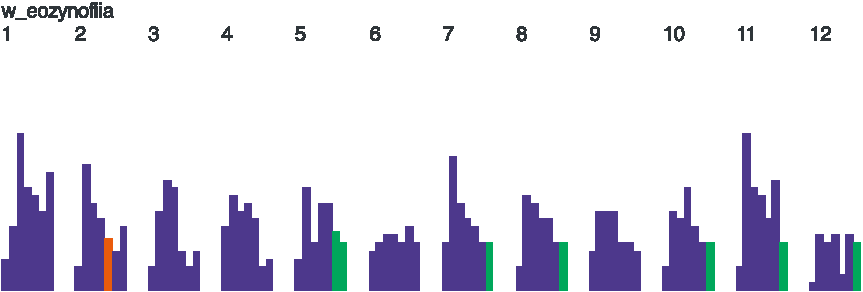
\includegraphics{fig9.pdf}}
\end{center}
\label{figure9}
\end{figure}

Figure 9 Example of data gap-filling
blue - measured values
red - interpolated values
green - extrapolated values


Of the three parameters describing menopause, one was selected as a binary variable - ``pokwitanie2'' (menopause2).
Additional parameters were calculated:
* For the spring check-ups
* Suma\_lekow\_diff
difference between the medication taken in current year and previous year
* Suma\_lekow\_mul
quotient of medication taken in current year and previous year
* suma\_lekow\_dic\_2{\ldots}32
sum of medications divided by subsequent powers of 2
for w3 divisor=2
for w4 divisor=4
{\ldots}
for wk divisor = 32
So the longer the treatment the less important the parameter value becomes compared with other parameters
* global
based on deterioration, i.e.\ the increase in amount of medication administered to patients compared with previous year
* stosunek\_pogorsz (deterioration)
relation of deterioration level to the length of treatment
this means that if a patient was treated for 5 years and had one deterioration period the parameter = 0.2
* stopien\_pogorszenia\_max
maximum deterioration
maximum value of quotient of sums of medication amount throughout the whole period of treatment
When preparing data for normalization, parameters value ranges and types were defined:


\begin{table}[htbp]
\begin{minipage}{\linewidth}
\setlength{\tymax}{0.5\linewidth}
\centering
\small
\caption{Table 3 Parameters value ranges and types}
\label{table3}
\begin{tabulary}{\linewidth}{@{}l@{}l@{}l@{}l@{}} \\ \toprule 
Name&type&min&Max \\\midrule
numer\_porzadkowy&int&1&80 \\
na\_co\_pierwsze\_chorowal&int&0&3 \\
pokwitanie2&int&0&7 \\
w\_czas\_choroby\_do\_it\_nos&int&2&10 \\
w\_czas\_choroby\_do\_it\_astma&int&0&10 \\
w\_eozynofilia&int&0&22 \\
grupa\_lub\_kontrola&int&1&2 \\
w\_eozynofilia\_bezw&int&0&2730 \\
w\_ecp&double&3.04&146.7 \\
w\_eozynofile&int&0&98 \\
w\_eozynofile\_zdegranulowane&int&0&5 \\
grupa\_pacjentow&int&1&3 \\
w\_fev&int&0&161 \\
w\_swiszczacy\_oddech&int&0&3 \\
w\_kaszel&int&0&7 \\
w\_dusznosc&int&0&3 \\
podzial\_na\_4\_grupy&int&1&4 \\
w\_swiad\_spojowek&int&0&3 \\
w\_lzawienie\_oczu&int&0&3 \\
w\_wyciek\_z\_nosa&int&0&3 \\
w\_zatkanie\_nosa&int&0&3 \\
w\_napady\_kichania&int&0&3 \\
w\_wysypki\_skorne&int&0&3 \\
w\_czestosc\_infekcji\_w\_roku&int&0&20 \\
w\_hospitalizacja\_\_w\_tyg&&& \\
w\_ig\_e\_swoiste\_trawy&double&0.8&157.9 \\
wiek\_w\_latach&int&5&15 \\
w\_ig\_e\_swoiste\_trawy\_klasa&int&2&5 \\
w\_max\_stezenie\_szczepionki&int&250&10000 \\
w\_dawka\_szczepionki&int&25&10000 \\
w\_czas\_trwania\_objawow&int&1&149 \\
w\_czas\_trwania\_max\_objawow&int&1&113 \\
testy\_trawy\_i&int&1&5 \\
testy\_trawy\_ii&int&1&5 \\
rozpoznanie&int&1&10 \\
natezenie\_astmy\_rozpoznanie&int&1&3 \\
w\_obciazajacy\_wywiad\_rodzinny&int&1&10 \\
obciazenie\_rodzinne&int&0&2 \\
w\_procent\_zmiennosci\_po\_beta&double&-22.0&92.0 \\
w\_poprawa\_kodowana&&& \\
w\_suma\_objawow&int&0&27 \\
w\_suma\_lekow&int&0&28 \\
miesiac\_urodzenia&int&1&12 \\
plec&int&1&2 \\
w\_antyhistaminiki&int&0&6 \\
w\_metyloksantyny&int&0&3 \\
w\_sterydy\_ogolnie&int&0&2 \\
w\_sterydy\_wziewnie&int&0&3 \\
w\_sterydy\_donosowo&int&0&3 \\
w\_kromoglikany\_wziewnie&int&0&3 \\
w\_kromoglikany\_donosowo&int&0&3 \\
w\_kromoglikany\_dospojowkowo&int&0&3 \\
w\_beta-mimetyki&int&0&3 \\
w\_betadrin\_miejscowo&int&0&3 \\
testy\_drzewa&int&1&5 \\
testy\_chwasty&int&1&5 \\
testy\_plesnie&int&1&4 \\
testy\_kurz&int&1&5 \\
testy\_dermpt&int&1&5 \\
testy\_dermfa&int&1&5 \\
ide\_c&double&11.6&2095.0 \\
ige\_swtr&double&0.8&52.0 \\
ige\_swtr\_klasa&int&2&5 \\
w\_czas\_choroby\_do\_it\_skora&int&1&8 \\
ige\_calk\_ponad\_norme&int&0&2 \\
ige\_swtr\_kl\_wieksze\_rowne\_2&int&0&2 \\
odczulani\_przez\_4\_lub\_5\_lat&int&1&2 \\
igec\_lub\_igesw&double&1.067901&812.086331 \\
igesw\_lub\_igec&double&0.001231&0.936416 \\
procent\_poprawa&int&0&2 \\
kryt\_igec\_800&int&0&2 \\
kryt\_igesw\_3&int&0&2 \\
kryt\_eobzw\_700&int&1&1 \\
w\_dlugosc\_choroby\_przed\_it&int&2&10 \\
w\_phadiatop&int&1&2 \\
w\_leukocytoza&int&3400&20300 \\
w\_liczba\_pol\_naplywowych&int&0&60 \\
w\_liczba\_pol\_nablonkowych&int&0&55 \\
w\_neutrofile&int&0&98 \\
w\_limfocyty&int&0&47 \\
w\_komorki\_kubkowe&int&0&59 \\
w\_komorki\_przypodstawne&int&0&57 \\
w\_sposob\_zluszczania&int&1&3 \\
w\_fef\_5-75&int&0&206 \\
w\_pefr&int&0&200 \\
w\_roznica\_miedzy\_objawami&&& \\
w\_ig\_e\_calkowite&double&11.6&2095.0 \\
w\_reakcje\_poszczepienne&int&1&1 \\
w\_hospitalizacja\_tyg&int&2&2 \\
pokwitanie&int&90&96 \\
w\_procent\_zmiennoci\_po\_beta&&& \\
kontrola\_dodatnia&int&2&20 \\
procent\_rozn\_sumy\_lekow&double&-320.0&100.0 \\
Poprawa&int&1&2 \\
roznica\_sumy\_objawow&int&-10&23 \\
procent\_rozn\_sumy\_objawow&double&-167.0&100.0 \\
rozn\_sumy\_lekow&int&-18&22 \\

		\bottomrule
	\end{tabulary}
\end{minipage}
\end{table}

\section{Discussion on the network selection}
\label{discussiononthenetworkselection}

Capabilities and effectiveness of neural networks depend on their types and topologies. Self-organizing networks have no application to problems with known expected results. Supervised networks come in several variants. The problem in question is finding a network predicting a single continuous parameter based on the input data that is compromised due to a patient's subjective testimony.
\textbf{Linear networks} - they divide the space with hyperplanes. They can classify input data as linear discriminating functions, or, for the regressing problems, create a plane common for all results. For the single dimension input vector it will be vector of the length similar to an arithmetic mean of the expected outputs set. In our case this variant has no application, since single output required is represented with a more complex function than a linear function.
\textbf{Multi Layer Perceptron (MLP) networks} - they are the most flexible type of neural networks, thanks to the flexibility of their structures, the number of layers and the number of neurons in layers. The price for this flexibility is the long time needed for training and the complex method of deciding upon their structure. Networks of this type are compatible with data containing measurement errors. Potentially, they may be a good fit for the problem defined.
Bayesian networks (Probabilistic Neural Networks and General Recurrent Neural Networks) - they are not very useful without an additional input data filtering to distinguish classes in place of continuous values. Moreover, these types of networks require large and representative input sets. Unfortunately, the available set is comprised of only 31 treated patients.


In order to choose the right type and the initial topology of a network, STATISTICA Neural Networks software suite was used. Its heuristic network architecture modeling capability was utilized. It is a module based on genetic algorithms. The smallest testing error with maintaining small validation error was achieved with MLP networks containing 3 hidden layers. Therefore, the SNN application heuristic analysis confirmed that the MLP type would be the most appropriate choice for the problem in question.
The research was conducted using a network trained with data coming from the ``interview'' and the results of tests ran during the first year of treatment - ``w1''. Deterioration\_level\_max (stopien\_pogorszenia\_max) was the expected value. This parameter provided satisfactory measure of patients' responsiveness to treatment. It was approved by the expert as a sufficient premise calculated by the system based on patient's data.
In order to maintain the same grouping for the training, validation and testing sets in subsequent trails, grouping was coded in additional field as ``elements\_category'' (kategoria\_elementu). Small training set - 32 patients undergoing desensitization - significantly limited the size of subsets, and therefore their representativity.
When training a network, an effort is made to minimize the training set error, so that the validating set error would also demonstrate this tendency\footnote{Precise definition of the error can be found in Chapter ``3.3.2. Delta Rule''}. The training is interrupted or modified, when the validating set error increases despite the training set error decreasing. This phenomenon signals the network's over-training. Additionally, when a system is also manipulating the architecture and additional testing set is needed to compare the effectiveness of architectures employed.
Mean square error is difficult to interpret in effectiveness and efficacy terms Therefore, a measure of quality is used.
Quality is defined as standard deviation of prediction errors divided by the standard deviation of the output values. The lower the value, the better the network is. 1 is the reference value, meaning that standard deviations of the errors and output values are equal. Further discussion on quality can be found in Chapter ``5.4.2. Results interpretation - quality of network''.


\begin{table}[htbp]
\begin{minipage}{\linewidth}
\setlength{\tymax}{0.5\linewidth}
\centering
\small
\caption{Table 4 Model comparison report  - SNN analysis  (for ``interview'' and '' w1'')}
\label{table4}
\begin{tabulary}{\linewidth}{@{}l@{}l@{}l@{}l@{}l@{}l@{}l@{}l@{}} \\ \toprule 
Type&Quality u&Quality w&Quality t&Error u&Error w&Error t&Training \\\midrule
MLP 12:12-20-14-1:1&0,380690&0,498705&1,190093&0,121202&0,094067&0,279640&BP100,CG20,CG0b \\
MLP 14:16-20-9-1:1&0,335765&0,607185&1,284842&0,150175&0,111574&0,299184&BP100,CG20,CG0b \\
MLP 14:16-20-14-1:1&0,582792&0,437756&1,116657&0,237672&0,105682&0,319769&BP100,CG20,CG0b \\
MLP 13:15-20-12-1:1&0,123424&0,389140&1,436121&0,035087&0,096008&0,319984&BP100,CG20,CG4b \\
MLP 7:7-6-7-1:1&0,665690&0,610414&1,447535&0,179719&0,116275&0,330673&BP100,CG20,CG0b \\
MLP 15:17-20-9-1:1&0,264581&0,618745&1,451452&0,138155&0,114406&0,338800&BP100,CG20,CG0b \\
MLP 15:17-10-1:1&0,231660&0,454477&1,200153&0,078188&0,109531&0,339726&BP100,CG20,CG4b \\
MLP 4:4-2-1:1&0,805073&0,552974&1,484017&0,219297&0,101591&0,344319&BP100,CG20,CG0b \\
MLP 4:4-3-1:1&0,811213&0,557543&1,456236&0,219032&0,104597&0,345654&BP100,CG20,CG0b \\
MLP 15:17-11-1:1&0,198413&0,540841&1,536433&0,104214&0,105661&0,349663&BP100,CG20,CG0b \\
MLP 4:4-2-1:1&0,780863&0,526773&1,507607&0,213295&0,096767&0,350154&BP100,CG20,CG0b \\
MLP 4:4-4-3-1:1&0,846051&0,552078&1,511738&0,229329&0,101746&0,351926&BP100,CG20,CG0b \\
MLP 5:5-5-1:1&0,710321&0,590508&1,579424&0,201146&0,108658&0,356409&BP100,CG20,CG0b \\
MLP 4:4-2-1:1&0,774417&0,513943&1,471086&0,210242&0,111574&0,359952&BP100,CG20,CG0b \\
MLP 12:14-17-11-1:1&0,162781&0,434490&1,639542&0,044071&0,110262&0,362816&BP100,CG20,CG7b \\
MLP 5:5-3-1:1&0,745334&0,538176&1,611793&0,209919&0,101412&0,363514&BP100,CG20,CG0b \\
MLP 11:13-12-1:1&0,260644&0,384830&1,004149&0,088035&0,097189&0,365674&BP100,CG20,CG4b \\
MLP 9:11-9-3-1:1&0,577114&0,623746&1,628581&0,156657&0,116341&0,367229&BP100,CG20,CG0b \\
MLP 16:18-19-11-1:1&0,350160&0,578795&1,654540&0,119055&0,112475&0,369242&BP100,CG20,CG0b \\
MLP 6:6-6-1:1&0,725854&0,615156&1,571625&0,196061&0,115624&0,370892&BP100,CG20,CG0b \\
MLP 4:4-2-4-1:1&0,704872&0,556447&1,585524&0,190951&0,116872&0,371313&BP100,CG20,CG2b \\
MLP 16:18-20-9-1:1&0,370024&0,542554&1,640938&0,182768&0,103323&0,372596&BP100,CG20,CG0b \\
MLP 6:6-6-1:1&0,917078&0,503426&1,327563&0,309476&0,115617&0,372698&BP100,CG20,CG0b \\
MLP 4:4-1-1:1&0,777665&0,426751&1,554062&0,210117&0,090829&0,373355&BP100,CG20,CG0b \\
MLP 5:5-5-1:1&0,771043&0,535800&1,659822&0,211810&0,104675&0,380664&BP100,CG20,CG0b \\
MLP 13:15-10-1:1&0,321735&0,546476&1,728790&0,104882&0,115704&0,381954&BP100,CG20,CG0b \\
MLP 11:11-19-12-1:1&0,590113&0,554898&1,629349&0,159363&0,110727&0,386118&BP100,CG20,CG0b \\
MLP 4:4-2-3-1:1&0,781493&0,465929&1,636549&0,211054&0,085820&0,391814&BP100,CG20,CG0b \\
MLP 15:17-20-13-1:1&0,211603&0,445799&1,783640&0,096922&0,115727&0,394946&BP100,CG20,CG0b \\
MLP 13:15-13-1:1&0,644430&0,377362&1,417624&0,217484&0,089714&0,396624&BP100,CG20,CG3b \\
MLP 13:13-20-12-1:1&0,031235&0,335306&0,960763&0,010541&0,112789&0,398376&BP100,CG3c,CG18b \\
MLP 8:10-9-1:1&0,477281&0,530189&1,811746&0,132172&0,114050&0,402044&BP100,CG20,CG0b \\
MLP 15:17-20-11-1:1&0,402919&0,482174&1,380107&0,136005&0,111542&0,404736&BP100,CG20,CG0b \\
MLP 16:18-20-14-1:1&0,107097&0,602723&1,866231&0,039450&0,112048&0,412420&BP100,CG18c,CG0b \\
MLP 16:18-20-16-1:1&0,192825&0,352507&1,899029&0,054619&0,069533&0,419564&BP100,CG20,CG0b \\
MLP 4:4-4-2-1:1&0,823711&0,416346&1,741773&0,222495&0,077512&0,426589&BP100,CG20,CG0b \\
MLP 6:8-4-1:1&0,734464&0,435643&1,564672&0,254432&0,101011&0,433064&BP100,CG20,CG0b \\
MLP 9:9-16-1:1&0,169805&0,582778&1,977887&0,045926&0,114559&0,437340&BP100,CG20,CG19b \\
MLP 10:12-9-1:1&0,716975&0,467183&1,650398&0,242616&0,109974&0,457386&BP100,CG10c,CG1b \\
MLP 13:15-15-1:1&0,162015&0,590399&2,083176&0,044870&0,116668&0,461158&BP100,CG20,CG1b \\
MLP 14:16-20-12-1:1&0,914459&0,432743&1,704218&0,382589&0,113037&0,474796&BP100,CG20,CG0b \\
MLP 12:14-8-1:1&0,806643&0,458358&1,473552&0,410181&0,110501&0,481491&BP100,CG20,CG0b \\
MLP 12:14-20-7-1:1&0,883554&0,439167&1,869964&0,311153&0,101850&0,522187&BP100,CG20,CG0b \\
MLP 7:7-8-1:1&0,978610&0,427022&1,853650&0,330255&0,100256&0,532399&BP100,CG20,CG0b \\
MLP 12:14-12-1:1&0,031931&0,445699&1,970777&0,010837&0,113703&0,547220&BP100,CG9c,CG38b \\
MLP 16:18-20-12-1:1&0,993051&0,413447&2,153515&0,335482&0,110189&0,594736&BP100,CG20,CG0b \\
MLP 12:12-20-11-1:1&0,992333&0,404479&1,933073&0,446052&0,102372&0,613625&BP100,CG2c,CG0b \\
MLP 12:14-18-2-1:1&0,015102&0,295528&2,372166&0,005203&0,090217&0,655342&BP100,CG20,CG111b \\
MLP 11:13-11-1:1&0,980947&0,502983&2,596820&0,331149&0,115505&0,722754&BP100,CG20,CG0b \\
MLP 14:16-12-1:1&0,740250&0,362849&3,830122&0,249813&0,102414&1,062333&BP100,CG19c,CG0b \\

		\bottomrule
	\end{tabulary}
\end{minipage}
\end{table}

Table 4 (\autoref{table4}) Notes: Quality u is the prediction quality for the training set. Similarly, `w' i `t' qualities are the validating set quality and the testing set quality. The lower the value the better network predicting for the given set. `t' set is used to compare architectures.


Two networks are highlighted in the table. First one has the smallest error for the training set. The second one has the lowest quality factor for this set.


\begin{figure}
\begin{center}
\resizebox{1\linewidth}{!}{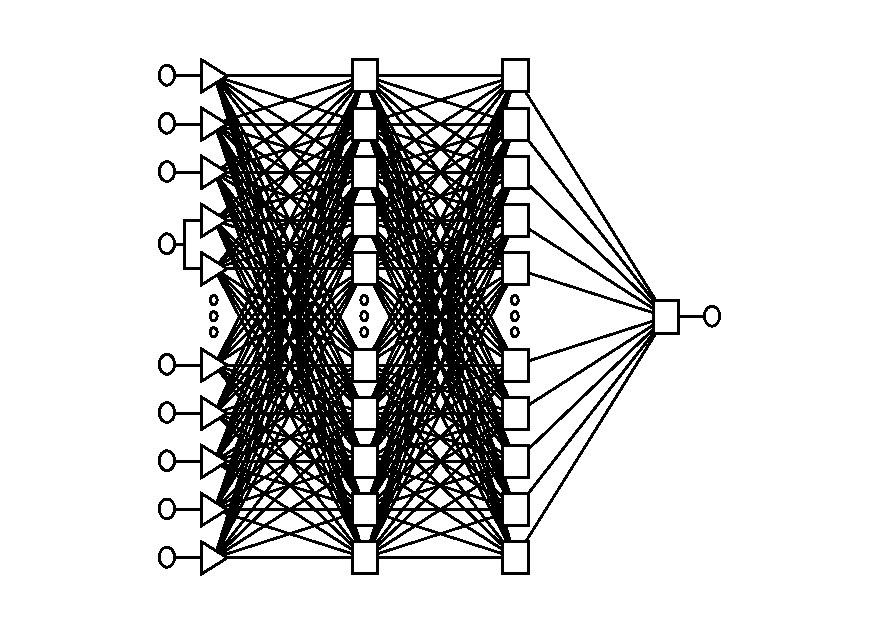
\includegraphics{fig10.pdf}}
\end{center}
\label{figure10}
\end{figure}

Figure 10 Structure with the lowest error and the best quality for the training set. MLP 14:16-20-14-1:1 stands for Multiple Layers Perceptron with 14 inputs, one output and two hidden layers.


As a test, an additional analysis was performed, with the data set expanded by the patients' results during the second year of treatment - ``w2''. Errors for validating and testing sets were smaller. At the same time the selected network also had better quality than the previous one. Unfortunately from the point of view of the patient the prognosis given only after having results of two year therapy is not very valuable. Further work was meant to improve the prediction accuracy for the network which only uses data from the interview and the initial check-ups results.


\begin{table}[htbp]
\begin{minipage}{\linewidth}
\setlength{\tymax}{0.5\linewidth}
\centering
\small
\caption{Table 5 Model comparison report - SNN analysis (for the interview, w1 and w2)}
\label{table5}
\begin{tabulary}{\linewidth}{@{}l@{}l@{}l@{}l@{}l@{}l@{}l@{}l@{}} \\ \toprule 
Type&Quality u&Quality w&Quality t&Error u&Error w&Error t&Training \\\midrule
MLP 38:40-40-26-1:1&0,836195&0,465419&1,627109&0,250976&0,086959&0,394338&BP100,CG20,CG0b \\
MLP 12:12-6-7-1:1&0,388333&0,466980&2,281773&0,105675&0,086839&0,536553&BP100,CG20,CG4b \\
MLP 35:37-40-6-1:1&0,709306&0,363941&1,118662&0,239400&0,086805&0,308959&BP100,CG20,CG1b \\
MLP 34:36-40-20-1:1&0,971769&0,460347&2,121890&0,290635&0,085301&0,573053&BP100,CG20,CG0b \\
MLP 39:41-40-28-1:1&0,117491&0,422299&1,393216&0,032230&0,084823&0,340834&BP100,CG20,CG7b \\
MLP 37:39-19-1:1&0,601358&0,458186&1,809214&0,164106&0,084525&0,469893&BP100,CG20,CG0b \\
MLP 17:19-9-1:1&0,635945&0,244268&1,493312&0,214677&0,084072&0,414894&BP100,CG20,CG1b \\
MLP 18:18-34-19-1:1&0,192059&0,425279&2,114409&0,052361&0,083869&0,471900&BP100,CG20,CG5b \\
MLP 29:31-26-1:1&0,085060&0,405942&1,803581&0,023062&0,082126&0,404179&BP100,CG20,CG12b \\
MLP 34:36-17-1:1&0,473714&0,335118&1,725211&0,128147&0,082008&0,394739&BP100,CG20,CG0b \\
MLP 29:29-40-18-1:1&0,078984&0,448008&2,350837&0,022681&0,081633&0,605806&BP100,CG20,CG18b \\
MLP 16:16-9-11-1:1&0,354839&0,432317&2,009292&0,109127&0,081372&0,444116&BP100,CG20,CG0b \\
MLP 14:14-17-1:1&0,459533&0,453861&1,391488&0,124181&0,081017&0,336539&BP100,CG20,CG4b \\
MLP 34:36-25-1:1&0,036789&0,405598&1,684664&0,010378&0,080602&0,382766&BP100,CG20,CG28b \\
MLP 39:41-27-1:1&0,065593&0,292724&1,518838&0,017757&0,080538&0,339172&BP100,CG20,CG29b \\
MLP 33:35-40-16-1:1&0,328557&0,417086&1,080160&0,089776&0,080095&0,284576&BP100,CG20,CG4b \\
MLP 23:25-19-1:1&0,464134&0,406869&1,995531&0,125523&0,079509&0,460588&BP100,CG20,CG1b \\
MLP 14:14-5-1:1&0,894167&0,198910&1,607734&0,301950&0,079314&0,481368&BP100,CG20,CG0b \\
MLP 32:34-40-8-1:1&0,601268&0,339794&1,116162&0,216758&0,079232&0,362675&BP100,CG20,CG1b \\
MLP 39:41-40-16-1:1&0,629805&0,374169&0,690159&0,171326&0,079172&0,184777&BP100,CG20,CG10b \\
MLP 13:15-37-12-1:1&0,447983&0,334896&2,023599&0,151498&0,077608&0,609311&BP100,CG20,CG20b \\
MLP 24:24-8-1:1&0,469401&0,299433&1,498087&0,161663&0,076724&0,452462&BP100,CG20,CG1b \\
MLP 34:36-15-1:1&0,059134&0,406987&1,237139&0,016843&0,076307&0,283994&BP100,CG20,CG10b \\
MLP 40:42-40-23-1:1&0,815075&0,414543&1,185614&0,223124&0,076161&0,296184&BP100,CG20,CG0b \\
MLP 35:37-23-1:1&0,529082&0,346977&2,481005&0,144451&0,075021&0,622625&BP100,CG20,CG0b \\
MLP 30:32-40-10-1:1&0,951601&0,307600&1,099561&0,321158&0,073996&0,307148&BP100,CG20,CG0b \\
MLP 37:39-40-18-1:1&0,134649&0,411785&1,659781&0,043799&0,073666&0,385314&BP100,CG20,CG2b \\
MLP 16:18-9-1:1&0,837666&0,314034&1,224892&0,282964&0,072827&0,347743&BP100,CG20,CG0b \\
MLP 34:34-40-15-1:1&0,680716&0,393129&1,546247&0,191123&0,071456&0,345588&BP100,CG20,CG0b \\
MLP 40:42-31-1:1&0,153255&0,393670&1,612541&0,042144&0,071454&0,365720&BP100,CG20,CG3b \\
MLP 34:36-24-1:1&0,553121&0,346357&1,808529&0,163637&0,069924&0,399824&BP100,CG20,CG0b \\
MLP 37:39-22-1:1&0,115546&0,384483&1,957599&0,031316&0,069131&0,437232&BP100,CG20,CG6b \\
MLP 35:37-23-1:1&0,097334&0,383827&1,539772&0,026497&0,068702&0,344871&BP100,CG20,CG16b \\
MLP 6:6-6-11-1:1&0,743648&0,377724&1,296814&0,235087&0,068229&0,286671&BP100,CG20,CG0b \\
MLP 35:37-40-15-1:1&0,033573&0,296309&1,502666&0,009432&0,067752&0,340602&BP100,CG20,CG12b \\
MLP 26:26-38-19-1:1&0,345694&0,325209&1,582741&0,094624&0,066279&0,356308&BP100,CG20,CG3b \\
MLP 36:38-25-1:1&0,443914&0,290156&1,258487&0,150887&0,065256&0,353508&BP100,CG7c,CG1b \\
MLP 25:27-9-1:1&0,457702&0,284045&2,034409&0,155510&0,064125&0,608277&BP100,CG20,CG1b \\
MLP 39:41-40-25-1:1&0,870786&0,305177&0,995518&0,239157&0,063939&0,249343&BP100,CG20,CG0b \\
MLP 22:24-20-1:1&0,714044&0,176330&1,806060&0,193043&0,063709&0,428589&BP100,CG20,CG0b \\
MLP 33:35-26-1:1&0,197774&0,336516&1,387059&0,053400&0,062835&0,308088&BP100,CG20,CG13b \\
MLP 18:20-38-19-1:1&0,501786&0,261710&1,833628&0,171049&0,059422&0,558767&BP100,CG20,CG3b \\
MLP 36:38-40-23-1:1&0,271958&0,308329&2,095973&0,080677&0,058506&0,486857&BP100,CG20,CG2b \\
MLP 33:35-31-1:1&0,007210&0,282025&1,238878&0,001948&0,050318&0,275998&BP100,CG20,CG21b \\
MLP 40:42-34-1:1&0,157288&0,257830&1,341501&0,042499&0,049886&0,307522&BP100,CG20c,CG0b \\
MLP 36:38-40-16-1:1&0,178566&0,248018&1,494768&0,049189&0,045384&0,330321&BP100,CG20,CG2b \\
MLP 36:38-28-1:1&0,079430&0,243449&1,683883&0,022425&0,044304&0,400428&BP100,CG20,CG19b \\
MLP 37:39-40-19-1:1&0,063921&0,216093&1,799112&0,017571&0,039021&0,411345&BP100,CG20,CG10b \\
MLP 34:36-20-1:1&0,274450&0,171115&1,467962&0,093004&0,038866&0,406097&BP100,CG4c,CG17b \\
MLP 32:34-40-23-1:1&0,225192&0,181894&1,757623&0,065976&0,032451&0,394853&BP100,CG20,CG2b \\

		\bottomrule
	\end{tabulary}
\end{minipage}
\end{table}

Highlighted is the network with the lowest Mean Square Error (MSE) of the testing set.


Based on those findings, data was further analyzed using a system designed by the author  - JIM (Java Immunotherapy Model, further presented in ``Chapter 6 JIM Computer analysis System''), in order to find the best possible network structure for the problem. The system employs genetic algorithms to choose the network's architecture and trains it utilizing the backpropagation algorithm with added local minima skipping, based on the annealing algorithm ~\cite{Joone:2005:Documentation}.


JIM recorded a full specification of a network in a single chromosome. The chromosome comprised of the following variables:


\begin{itemize}


\item Inputs subset - a bit map of decision whether to use a given input

\item First hidden layer width

\item Second hidden layer width

\item Third hidden layer width

\item Type of layers used:

\item Hyperbolic tangent

\item Sigmoid

\item Logarithmic

\item learningRate - the speed of learning

\item momentum - initial speed of learning
\end{itemize}

Structure selection process consisted of evolving a population made of 60 members in 10 generations. A roulette method of selection was employed. The adaptation function arguments included:


\begin{itemize}


\item RMSE
the most important of the adaptation function value are reciprocal of RMSE

\item Inputs number
Subsequent bits are reciprocal of the inputs number

\item The sum of the hidden neurons
Last bits are reciprocal to the sums of the hidden layers neurons
\end{itemize}

\section{Interpretation of results - network quality}
\label{interpretationofresults-networkquality}

SNN application employs ``error'' and ``quality'' parameters to describe a given network. Those are calculated for the training, validation and testing sets.
The ``Error'' is the Mean Square Error discussed in the introduction. ``Quality'' of a network working regression problems is defined as standard deviation of prediction errors divided by the standard deviation of the output values:


\begin{equation}
J=\frac{{\sigma }_{p}}{{\sigma }_{w}}
\end{equation}


$ {\sigma }_{p}$ - standard deviation of the prediction errors set
$ {\sigma }_{w}$ - standard deviation of the outputs set


For finite populations, the standard deviation is calculated using:


\begin{equation}
\sigma =\sqrt{\frac{\sum _{i=1}^{N}{({x}_{i}-\mu )}^{2}}{N(N-1)}}
\end{equation}


$ {x}_{i}$ - value of characteristic in population
$ \mu $ - expected value
$ N$ - population number


The expected value for a population with constant probability is the mean population value. This means that the mean square difference of prediction error and mean prediction error is compared with the mean square difference between data and their mean value.
Independent value of the standard deviation of the prediction errors set is not informative; therefore it needs to be compared with the standard deviation of the output values set. The starting point of comparing those two values could be a network model predicting constant output value equal to the mean output value of the data set. That model is wrong, since it is independent of the input values. Standard deviation of the prediction errors set will be equal to the standard deviation of the output set. The quotient will equal 1.
For a desirable network correctly modeling the assignment, this value has to be significantly lower than 1. Prediction spread has to be lower than the output data spread. It is accepted that ~\cite{Statistica:2004} the quality factor of 0.1 means a good regression.


\section{Comparison of networks}
\label{comparisonofnetworks}

The network with the lowest error of the testing set suggested by SNN is ``MLP 12:12-20-14-1:1''. The network with the best quality is ``MLP 13:13-20-12-1:1''. The comparison of those networks is presented in Table 6 (\autoref{table6}).


\begin{table}[htbp]
\begin{minipage}{\linewidth}
\setlength{\tymax}{0.5\linewidth}
\centering
\small
\caption{Table 6 Comparison of the best networks}
\label{table6}
\begin{tabulary}{\linewidth}{@{}l@{}l@{}l@{}l@{}l@{}l@{}l@{}l@{}} \\ \toprule 
Type&Quality u&Quality w&Quality t&Error u&Error w&Error t&training \\\midrule
MLP 13:13-20-12-1:1&0,031235&0,335306&0,960763&0,010541&0,112789&0,398376&BP100,CG3c,CG18b \\
MLP 12:12-20-14-1:1&0,380690&0,498705&1,190093&0,121202&0,094067&0,279640&BP100,CG20,CG0b \\

		\bottomrule
	\end{tabulary}
\end{minipage}
\end{table}

Networks were trained using the backpropagation algorithm and the conjugate gradient algorithm. First network has a quality factor value of 0.96 for the teting set, so its quality is nearing 1. For a network working regression problems the quality is defined as a quotient of standard deviations of prediction errors and standard deviations of data. A value of 1 of this factor means that the standard deviation of prediction errors is comparable to the standard deviation of data. This means that the network gives out results of quality comparable to those of a network modelling the mean output values.


\begin{table}[htbp]
\begin{minipage}{\linewidth}
\setlength{\tymax}{0.5\linewidth}
\centering
\small
\caption{Table 7 Comparison of expected values with the prediction of  best networks for the testing set}
\label{table7}
\begin{tabulary}{\linewidth}{@{}l@{}l@{}l@{}l@{}l@{}l@{}} \\ \toprule 
No&Expected values&MLP 13:13-20-12-1:1 Prognosis&MLP 13:13-20-12-1:1 Error&MLP 12:12-20-14-1:1  Prognosis&MLP 12:12-20-14-1:1 Error \\\midrule
1&0,000000&-0,043314&0,043314&-0,118149&0,118149 \\
2&0,000000&-0,278319&0,278319&-0,001623&0,001623 \\
3&0,375000&0,186607&0,188393&0,262080&0,112920 \\
4&0,250000&0,138617&0,111383&0,104553&0,145447 \\
5&0,444444&-0,080890&0,525334&-0,154654&0,599098 \\
6&0,000000&0,055671&0,055671&-0,060779&0,060779 \\
7&0,000000&-0,295691&0,295691&-0,074360&0,074360 \\

		\bottomrule
	\end{tabulary}
\end{minipage}
\end{table}

Looking at the cases, high level of errors is apparent in values predicted for the testing set. \textbf{Predicted was the maximum deterioration of patient's condition in one year, throughout the whole period of treatment.}
The research aim was to devise of a system supporting doctors when deciding on whether patients qualify for treatment. After consulting with an expert - dr Ewa Cichocka-Jarosz - on quality of the results, a hypothesis was formulated on predicting \textbf{whether deterioration will occur}. A classifying threshold was established at 7.5\%. It means that, from the point of view of a doctor, a deterioration of 7.5\% is not burdensome for the patients, measured in the amount of medication taken in order to function normally.


\begin{table}[htbp]
\begin{minipage}{\linewidth}
\setlength{\tymax}{0.5\linewidth}
\centering
\small
\caption{Table 8 Comparison of classifier expected values with predictions of best networks for the testing set}
\label{table8}
\begin{tabulary}{\linewidth}{@{}l@{}l@{}l@{}l@{}l@{}l@{}l@{}l@{}l@{}} \\ \toprule 
No&Expected Values&Had deterioration not occured?&MLP 13: 13-20-12-1:1&Had deterioration not occured?&Was prediction correct?&MLP 12: 12-20-14-1:1&Had deterioration not occured?&Was prediction correct? \\\midrule
1&0,000000&TRUE&-0,043310&TRUE&TRUE&-0,118150&FALSE&\textbf{FALSE} \\
2&0,000000&TRUE&-0,278320&FALSE&\textbf{FALSE}&-0,001620&TRUE&TRUE \\
3&0,375000&FALSE&0,186607&FALSE&TRUE&0,262080&FALSE&TRUE \\
4&0,250000&FALSE&0,138617&FALSE&TRUE&0,104553&FALSE&TRUE \\
5&0,444444&FALSE&-0,080890&FALSE&TRUE&-0,154650&FALSE&TRUE \\
6&0,000000&TRUE&0,055671&TRUE&TRUE&-0,060780&TRUE&TRUE \\
7&0,000000&TRUE&-0,295690&FALSE&\textbf{FALSE}&-0,074360&TRUE&TRUE \\

		\bottomrule
	\end{tabulary}
\end{minipage}
\end{table}

Wrong predictions were identified. The first network was mistaken on two patients: no.2 and no.7. The prediction success rate therefore was 71.5\%. The second network failed with one patient - no.1. The success rate was 85.8\%.


\begin{table}[htbp]
\begin{minipage}{\linewidth}
\setlength{\tymax}{0.5\linewidth}
\centering
\small
\caption{Table 9 Comparison of expected values with the predictions of the best networks for the validating set}
\label{table9}
\begin{tabulary}{\linewidth}{@{}l@{}l@{}l@{}l@{}l@{}l@{}l@{}l@{}l@{}} \\ \toprule 
No&Expected Value&MLP 13:13-20-12-1:1 prognosis&MLP 13:13-20-12-1:1 error&MLP 12:12-20-14-1:1 prognosis&MLP 12:12-20-14-1:1 error \\\midrule
1&0,166667&0,251501&0,084834&0,314250&0,147583 \\
2&0,363636&0,327791&0,035845&0,435394&0,071758 \\
3&0,333333&0,354619&0,021286&0,297487&0,035846 \\
4&0,000000&0,075336&0,075336&0,012003&0,012003 \\
5&0,000000&0,073820&0,073820&0,121240&0,121240 \\
6&0,000000&0,028417&0,028417&0,036233&0,036233 \\
7&0,285714&0,422500&0,136786&0,306602&0,020888 \\

		\bottomrule
	\end{tabulary}
\end{minipage}
\end{table}

\begin{table}[htbp]
\begin{minipage}{\linewidth}
\setlength{\tymax}{0.5\linewidth}
\centering
\small
\caption{Table 10 Comparison of the classifier expected values with the best networks' predictions for the validating set}
\label{table10}
\begin{tabulary}{\linewidth}{@{}l@{}l@{}l@{}l@{}l@{}l@{}l@{}l@{}l@{}} \\ \toprule 
No&Expected values&Had deterioration not occured?&MLP 13: 13-20-12-1:1&Had deterioration not occured?&Was prediction correct ?&MLP 12: 12-20-14-1:1&Had deterioration not occured?&Was prediction correct ? \\\midrule
1&0,166667&FALSE&0,251501&FALSE&TRUE&0,31425&FALSE&TRUE \\
2&0,363636&FALSE&0,327791&FALSE&TRUE&0,435394&FALSE&TRUE \\
3&0,333333&FALSE&0,354619&FALSE&TRUE&0,297487&FALSE&TRUE \\
4&0,000000&TRUE&0,075336&FALSE&\textbf{FALSE}&0,012003&TRUE&TRUE \\
5&0,000000&TRUE&0,07382&TRUE&TRUE&0,12124&FALSE&\textbf{FALSE} \\
6&0,000000&TRUE&0,028417&TRUE&TRUE&0,036233&TRUE&TRUE \\
7&0,285714&FALSE&0,4225&FALSE&TRUE&0,306602&FALSE&TRUE \\

		\bottomrule
	\end{tabulary}
\end{minipage}
\end{table}

Failed prognosis were highlighted. The hypothesis on predicting by using a classifier gives the prognosis precision for the validating set at 86\%.


\begin{table}[htbp]
\begin{minipage}{\linewidth}
\setlength{\tymax}{0.5\linewidth}
\centering
\small
\caption{Table 11 Comaprison of expected values with the predictions of the best networks for thetraining set}
\label{table11}
\begin{tabulary}{\linewidth}{@{}l@{}l@{}l@{}l@{}l@{}l@{}} \\ \toprule 
No&Expected Value&MLP 13:13-20-12-1:1 prognosis&MLP 13:13-20-12-1:1 error&MLP 12:12-20-14-1:1 prognosis&MLP 12:12-20-14-1:1 Error \\\midrule
1&0,000000&-0,006501&0,006501&0,023957&0,023957 \\
2&0,000000&0,007466&0,007466&-0,005603&0,005603 \\
3&0,000000&0,000447&0,000447&0,023219&0,023219 \\
4&0,181818&0,178565&0,003253&0,231627&0,049809 \\
5&0,000000&-0,012607&0,012607&-0,031640&0,031640 \\
6&0,272727&0,267516&0,005211&0,274245&0,001518 \\
7&0,600000&0,602406&0,002406&0,589727&0,010273 \\
8&0,000000&-0,012214&0,012214&0,004326&0,004326 \\
9&0,000000&0,004209&0,004209&-0,007642&0,007642 \\
10&0,461538&0,455638&0,005900&0,429161&0,032377 \\
11&0,125000&0,130785&0,005785&0,061191&0,063809 \\
12&0,000000&0,006553&0,006553&-0,014312&0,014312 \\
13&0,333333&0,338616&0,005283&0,331784&0,001549 \\
14&0,333333&0,331775&0,001558&0,283209&0,050124 \\
15&0,000000&0,013126&0,013126&-0,000022&0,000022 \\
16&0,666667&0,669622&0,002955&0,634604&0,032063 \\

		\bottomrule
	\end{tabulary}
\end{minipage}
\end{table}

\begin{table}[htbp]
\begin{minipage}{\linewidth}
\setlength{\tymax}{0.5\linewidth}
\centering
\small
\caption{Table 12 Comparison of the classifier expected values with the best networks' predictions for the training set}
\label{table12}
\begin{tabulary}{\linewidth}{@{}l@{}l@{}l@{}l@{}l@{}l@{}l@{}l@{}l@{}} \\ \toprule 
No&Expected values&Had deterioration not occured?&MLP 13: 13-20-12-1:1&Had deterioration not occured?&Was prediction correct&MLP 12: 12-20-14-1:1&Had deterioration not occured?&Was prediction correct \\\midrule
1&0,000000&TRUE&-0,006500&TRUE&TRUE&0,023957&TRUE&TRUE \\
2&0,000000&TRUE&0,007466&TRUE&TRUE&-0,005603&TRUE&TRUE \\
3&0,000000&TRUE&0,000447&TRUE&TRUE&0,023219&TRUE&TRUE \\
4&0,181818&FALSE&0,178565&FALSE&TRUE&0,231627&FALSE&TRUE \\
5&0,000000&TRUE&-0,012610&TRUE&TRUE&-0,031640&TRUE&TRUE \\
6&0,272727&FALSE&0,267516&FALSE&TRUE&0,274245&FALSE&TRUE \\
7&0,600000&FALSE&0,602406&FALSE&TRUE&0,589727&FALSE&TRUE \\
8&0,000000&TRUE&-0,012210&TRUE&TRUE&0,004326&TRUE&TRUE \\
9&0,000000&TRUE&0,004209&TRUE&TRUE&-0,007642&TRUE&TRUE \\
10&0,461538&FALSE&0,455638&FALSE&TRUE&0,429161&FALSE&TRUE \\
11&0,125000&FALSE&0,130785&FALSE&TRUE&0,061191&TRUE&\textbf{FALSE} \\
12&0,000000&TRUE&0,006553&TRUE&TRUE&-0,014312&TRUE&TRUE \\
13&0,333333&FALSE&0,338616&FALSE&TRUE&0,331784&FALSE&TRUE \\
14&0,333333&FALSE&0,331775&FALSE&TRUE&0,283209&FALSE&TRUE \\
15&0,000000&TRUE&0,013126&TRUE&TRUE&-0,000022&TRUE&TRUE \\
16&0,666667&FALSE&0,669622&FALSE&TRUE&0,634604&FALSE&TRUE \\

		\bottomrule
	\end{tabulary}
\end{minipage}
\end{table}

One wrong prognosis is highlighted in the above table. All predictions of the first network were correct for the training set. For the second network 1 (of16) predictions had a slight error. The prognosis was that desensitizing of the no.11 patient will not result in deterioration. However, deterioration did occur, albeit slight. This means that the first network had a prediction success rate of 100\%, and the second one of 93.7\%.
Analysis conducted in the JIM system confirmed the SNN results. JIM was markedly slower than SNN and had a strong tendency to learn a single output value, which was the mean arithmetic of the predictions. Interesting was the advantage that the hyperbolic tangent neural networks had over logarithmic and sigmoidal threshold functions network when modeling the problem.


\section{The interpretation of input parameters}
\label{theinterpretationofinputparameters}

From the perspective of the input parameters selection, ``MLP 13:13-20-12-1:1'' network is the most interesting one. Reducing the number of parameters to 13 in ``MLP 12: 12-20-14-1:1'' lowers the quality.


\begin{table}[htbp]
\begin{minipage}{\linewidth}
\setlength{\tymax}{0.5\linewidth}
\centering
\small
\caption{Table 13}
\label{table13}
\begin{tabulary}{\linewidth}{@{}l@{}l@{}l@{}l@{}l@{}l@{}l@{}l@{}} \\ \toprule 
Type&Quality u&Quality w&Quality t&Error u&Error w&Error t&Training \\\midrule
MLP 13:13-20-12-1:1&0,031235&0,335306&0,960763&0,010541&0,112789&0,398376&BP100,CG3c,CG18b \\

		\bottomrule
	\end{tabulary}
\end{minipage}
\end{table}

Network parameters:


Interview group:


\begin{itemize}


\item wiek\_w\_latach (age in years)

\item rozpoznanie (diagnosis)

\item natezenia\_astmy\_rozpoznanie (asthma severity diagnosed)

\item w\_czas\_choroby\_do\_it\_nos (lenght of sickness - nose)

\item w\_czas\_choroby\_do\_it\_astma (lenght of sickness - asthma)

\item w\_obciazajacy\_wywiad\_rodzinny (indicative family history interview)

\item obciazenie\_rodzinne (family history)
\end{itemize}

Group w1:


\begin{itemize}


\item eozynofilia (eosinophiles)

\item eozynofilia\_bezw (absolute eosinophiles)

\item w\_ecp

\item w\_eozynofile\_zdegranulowane (degranulated eosinophiles)

\item w\_fev

\item w\_procent\_zmiennosci\_po\_beta (change percentage after beta)
\end{itemize}

\part{JIM Computer Analysis System}
\label{chapter6}

The development of the JIM system took place simultaneously with the data analysis. Its main task was to convert the data into format compatible with the analyzing and reasoning system. The conversion also included data filtering and conducting an additional expert interview. Additionally, the system was to make possible the selection and training of the network independently of the SNN software.
Full system specifications are included in ``Appendix A: Specification of the JIM system requirements''. Additional CD contains the code.


System functionality includes:


\begin{itemize}


\item Initial processing of the data and expert knowledge

\item Recording patients' data in an xml open format files

\item Automatic knowledge acquisition from data

\item Heuristic selection of appropriate network architecture best fitted for the type of data

\item Inferring on patients based on previously acquired knowledge - the outcome of this phase is recorded into xml format.
\end{itemize}

\chapter{Presentation of potentially useful tools for implementing the selected inference engine}
\label{presentationofpotentiallyusefultoolsforimplementingtheselectedinferenceengine}

\section{STATISTICA}
\label{statistica}

STATISTICA\footnote{http://www.statsoft.com/} is an integrated data analysis software suite. The neural network module first appeared in version no.5, as an independent application. It has been since integrated with the suite starting from version 6. It is available in the STATISTICA Neural Network package. There is also a STATISTICA Neural Networks Code Generator, which allows exporting of the generated network into external C/C++ code or into PMML (Predictive Model Markup Language). The package implements many network training algorithms and additionally contains own heuristics for choosing the right architecture for the given problem.


\section{SNNS - Stuttgart Neural Network Simulator}
\label{snns-stuttgartneuralnetworksimulator}

Available under GNU license for research purposes. Last version dates back to 1998. Later, the interface implementation in Java appeared.\footnote{http://www-ra.informatik.uni-tuebingen.de/SNNS/}


\section{CILib - Computational Intelligence Library}
\label{cilib-computationalintelligencelibrary}

Library implementing a host of artificial intelligence problems.\footnote{http://cilib.sourceforge.net/} Maintained by the Pretoria University, South Africa. It covers:
* Swarm intelligence
* Evolutionary algorithms
* Neural networks
* Artificial immunological systems
* Fuzzy logic


\section{JAGA - Java API for Genetic Algorithms}
\label{jaga-javaapiforgeneticalgorithms}

A relatively new project, still in the beta phase. Included analytical tools make it promising.\footnote{http://www.jaga.org/}


\section{JGAP - Java Genetic Algorithms Package}
\label{jgap-javageneticalgorithmspackage}

Version 1.0 of the package means it is now fully functional.\footnote{http://jgap.sourceforge.net/} Implemented are the basic genes and operations. It is interesting since it can be integrated with JOONE. Has the OSI\footnote{http://opensource.org/docs/certification\_mark.php} certification.


\section{JOONE - Java Object Oriented Neural Engine}
\label{joone-javaobjectorientedneuralengine}

This library is currently intensely developed. It implements neural networks by building them from readymade elements. User chooses the layer type, number of connections and so on separately.\footnote{http://www.jooneworld.com/}


There exist a complete graphical environment, in which testing and creating networks is possible. Networks are trained exclusively by back propagation of errors. The DynamicAnnealing module modifies the training parameters dynamically, which optimizes the whole process. 1.1.0 is the current version, with improvements of approx. 35\% over the previous one and supporting multi-processor computers. It is capable of parallel computations within a cluster. Capability of storing networks in the ANNML (Artificial Neural Network Markup Language) is planned. ANNML is an XML based PNML expansion.


\section{Saxon}
\label{saxon}

Referential implementation\footnote{http://saxon.sourceforge.net/} of  XSLT 2.0, XPath 2.0 and XQuery 1.0.


\section{AppLib - Approximation Library for Java}
\label{applib-approximationlibraryforjava}

Project developed under Alexander I. Rozhenko.\footnote{http://www.sscc.ru/matso/rozhenko/applib/} It implements interpolations using the splines method.


\section{Eclipse}
\label{eclipse}

Free programming environment for the Java language. It has evolved into a universal programming environment. IBM is the project's patron.\footnote{http://www.eclipse.org/}


\chapter{Discussion on the system selected from the perspective of tools available}
\label{discussiononthesystemselectedfromtheperspectiveoftoolsavailable}

The initial objective was to model knowledge on patients undergoing desensitization treatment in a neural network, by using the STATISTICA Neural Networks software. The network was then to be exported into an independent application. Unfortunately, exporting was only available in STATISTICA Neural Networks Code Generator. License cost was too high for the project's budget.
Alternative plan consisted of finding a flexible environment for working on data and neural networks. It was important that the tools and libraries used were licencensed as open source: GNU GPL or BSD variant.


During initial stages of the project it was decided that all possible data would be stored in XML format and that, when feasible, the data operations will be transformations of the XSLT. Initial conversion of source data from the CSV format into XML was performed using Perl.


The utilization of XML was useful due to the availability of freeware editors and the possibility of defining a coherent data processing methodology. Some charts used in this thesis are conversions of XML data into SVG vector graphics (XML). To reduce the cost of the typical programming errors and to make the project platform-independent, Java was chosen as the implementation language.
XSLT 2.0 was used for data transformation. Xpath 1.0, being a part of XSLT 1.0, did not allow addressing elements by the names contained in variables.  During developing of the system, Saxon was the only library capable of XSLT 2.0 transformations.


Initial data processing required data gap-filling. Interpolation using splines was selected as a method, due to the medical data characteristics. Only complete data could be used for training of networks.


The neural networks library had to be fast and as flexible as possible. There was an additional risk that the personal computer used for training network would be too slow. The requirements were met by the JOONE project. It was a safe solution, since it also featured extensions for distributed computing (JOONE-distributed). The code for network activation is so small that it can potentially be run on PDA-type devices, which is an interesting development path for the system. For the needs of the system, the JOONE library was expanded with XML input and XHTML output support.


The next phase required a tool for the network topology selection. CILib, JAGA and JGAP were considered. CILib implemented genetic algorithms in narrowest capacity. JAGA was still in beta and at the time of module's implementation a sample code using the library was missing. JGAP needed expanding with Double gene. Therefore, a org.jim.election.genes.DoubleGene class was created, consisting of 126 Non Commented Lines of Code. JGAP had good documentations and examples.


\begin{table}[htbp]
\begin{minipage}{\linewidth}
\setlength{\tymax}{0.5\linewidth}
\centering
\small
\caption{Table 14 Summary of technologies employed}
\label{table14}
\begin{tabulary}{\linewidth}{@{}llll@{}} \\ \toprule 
Name/Description&Choice&Rationale&Remarks \\\midrule
Stage 1: Converting textual data into xml&perl&Language optimized for textual data processing& \\
Stage 2: Filtering data based on the expert advice&xslt&Language optimized for xml-$>$xml conversion&After expert's conclusions were written up, an xml file was created \\
Stage 3: Data gap-filling&java, xslt&Part of data processing was convenient in xslt. Interpolation using secondary splines. Existing java numerical libraries were used& \\
Stage 4: Knowledge extraction from data&java&Large number of libraries, transferability&Neural network library selected: joone, Network architecure selection library chosen: jgap \\
Stage 5: Infering&java&Infering means transoforming the xml patients' data into output data (conlusions), by using an engine and knowledge. Stage 5 shares the code with Stage 4.& \\
Transformation coordination tool&ant&Native xslt, java support (compiling, method developing)& \\
ANN library&Joone&Open, well documented. Capacity for distributed computing. Easy implementation of custom input/output layers&Library has been modified by expanding with xml input data support \\
Data imaging&xslt, svg&svg is an xml expression of graphical objects. Transformation of xml data in svg by using xslt is natural.& \\
Transformation&mainly xslt 2.0&Well defined standard. Capable of converting xml into any variation of xml.&Objective was to create some appendixes and figures as xml-$>$pdf conversion \\
Xslt transformation&saxon&Closest implementation of xslt 2.0 (working draft). The author of library  collaborates on defining the standard& \\
Data format&xml&Univarsal format. Large number of libraries and editors interpreting and checking the syntax compatibility.& \\

		\bottomrule
	\end{tabulary}
\end{minipage}
\end{table}

\chapter{Build report}
\label{buildreport}

User interface is available through the Ant tool. JIM system achieves multiple ``targets'', which are the subsequent data processing stages. Ant allowed for transparent depicting of the dependency relations of processing stages


\begin{figure}
\begin{center}
\resizebox{1\linewidth}{!}{\includegraphics{fig11.png}}
\end{center}
\label{figure11}
\end{figure}

Figure 11 Relations of the transformations products


\section{Completer}
\label{completer}

The module responsible for data-gaps filling and calculating additional factors


\section{Range Selector}
\label{rangeselector}

The module calculating the data ranges, so that they could be normalized before the training. Additionally, the module recognized whether a parameter had continuous or discrete values and whether it was a classifier.


\section{Teacher}
\label{teacher}

Teacher of a network with a predetermined structure


\section{Executor}
\label{executor}

This module activated the network with given data


\section{NetworkArchitectureElector}
\label{networkarchitectureelector}

The module heuristically selected the networ's architecture, by employing genetic algorithms. The resulting architecure were recorded as chromosomes.


\section{ChromosomeTeacher}
\label{chromosometeacher}

The module trained the network based on the architecture stored in the chromosome.


The configuration of the all the above modules is contained in the jim.properties file. It contains information on: the localization of data file (data\_input.xml), field normalization values file (pola\_normalizacja), network parameters file (serialized\_network), and file storing the inference results (execution\_output\_html). Additionally, it contains a matrix specification of input and predicted data stored as xpath format queries.  Input data matrix for the training set consists of patients selected with the ``learning-xpath'' query and  the parameters describing patients selected with ``input\_xpath'' query. Output parameters are defined in the ``output\_xpath'' query. Similarly, the ``testing\_xpath'' query defines the patients testing the network, and the ``validating\_xpath'' defines patients validating the network.


Sample config file:


execution\_output\_html=./data.output/store.html
data\_input\_xml=./data.preprocessed/dane-completed.xml
pola\_normalization=./data.conf/pola-ranges.xml
serialized\_network=./data.nn/store.jnn
input\_xpath={\itshape [self$\backslash$:$\backslash$:wywiad or self$\backslash$:$\backslash$:w1]/}
output\_xpath=computed/stopien\_pogorszenia\_max
learning\_xpath=//pacjenci/pacjent[(position() $<$$\backslash$= 32) and ((position() mod 5) $>$ 1)]
testing\_xpath=//pacjenci/pacjent[(position() $<$$\backslash$= 32) and ((position() mod 5) $\backslash$= 1)]
validating\_xpath=//pacjenci/pacjent[(position() $<$$\backslash$= 32) and ((position() mod 5) $\backslash$= 0)]


\section{Summary}
\label{summary}

The system starts by converting the existing patients' database into xml format. Since that moment, all operations are transformations of data from xml to xml. Doctor interview was recorded as xml and merged with the existing data by a relevant transformation. Thanks to that, the system is very flexible and, with little work, allows for processing of any other type of data requiring a prediction of continuous values.


The system implements all the mentioned requirements except those concerning the graphical interface. The complexity of the task was too high to start working on it, when the data available for analysis would not allow for a proper regression.


\part{Concluding remarks}
\label{chapter7}

The aim of the project was to extract knowledge from existing data on immunotherapy, in order to develop a system supporting doctors in decisions concerning recommending patients for this costly treatment. Conducted researched demonstrated that the number of patients, on whom data was available, was too small for effective neural network utilization. However, the network built does provide a measure of support for doctors, albeit smaller than it was initially planned.


The JIM system developed combines ``open source'' components and allows for heuristic analysis, visualizations and inference based on treatment data. After adding more patients to the data set, it will be capable of quick analysis of prognoses.


Thanks to its flexible structure it is possible to adapt it to different problems requiring an optimization of the network's structure.
Two universal components were developed for the needs of the system, allowing for flexible utilization of the xml data as inputs to neural networks based on JOONE library. They will be included as integral parts of the next version of this library.


Learning about immunology and the defense mechanisms of living organisms proved to be very engaging and stimulating for the author. It is fascinating how little does medicine know about the immunotherapy's mechanisms. Another challenging aspect of the research was sorting the flows of data and results to proceed from the experimental stage to sequential processing. The most interesting part, however, was the network selection process. It was difficult to reconcile the limitations of the genetic algorithms of the simulating library with the large amount of parameters defining a network. It was also difficult to define the ``stopping condition'' of network training, to allow for calculating the adaptation function in real time. Yet overcoming these obstacles proved very satisfying.


In case of obtaining more representative data set, e.g.\ data on few hundred patients undergoing desensitization, the existing solutions are worth developing further by:


\begin{itemize}


\item in respect to the neural network:

\item implementing training algorithms alternative to backpropagation

\item increasing the time of network evolution

\item monitoring the process of population evolution

\item proceeding from initiating the network with random data to initial training by using a genetic algorithm [Yao, 1993],

\item neural network could be stored in portable Predictive Model Markup Language format

\item adding further inference engines

\item not limiting the analysis only to neural networks

\item ideally, at least one engine synthesizing conclusions of other engines should be developed

\item possible implementation would consist of several parallel engines, which would present a combined conclusion to users

\item developing a graphical user interface

\item it would improve data entry and allow for managing patients' database

\item expanding the system with the HL7\footnote{http://www.hl7.org/} interface

\item it would allow o integrate the system with other existing medical solutions
\end{itemize}

\part{JIM Requirements specification}
\label{appendixa}

\chapter{Meta-requirements}
\label{meta-requirements}

\section{[JIM-HRS-0001]}
\label{jim-hrs-0001}

System's objective is to support an immunologist when recommending patients for SIT therapy


\section{[JIM-HRS-0002]}
\label{jim-hrs-0002}

Inference of the system can be based on any heuristic embedded as an exchangeable plug-in


\section{[JIM-HRS-0003]}
\label{jim-hrs-0003}

System should be based on free software and not require any license fees. Suggested licenses are:
a) GNU GPL
b) GNU LGPL
c) BSD
d) Apache


\section{[JIM-HRS-0004]}
\label{jim-hrs-0004}

The system should have full functionality at the command line level, so it can be easily embedded in existing solutions


\section{[JIM-HRS-0005]}
\label{jim-hrs-0005}

Optionally, the system should have a graphical user interface


\section{Specification of the software requirements}
\label{specificationofthesoftwarerequirements}

\section{[JIM-SRS-0100]}
\label{jim-srs-0100}

Software will be based on open standards


\section{[JIM-SRS-0200]}
\label{jim-srs-0200}

Java will be the main language used; parts of logic could be implemented in XSL 2.0. When using other languages, attention should be placed to their portability. Languages used are defined in the following sub-requirements:


\section{[JIM-SRS-0201]}
\label{jim-srs-0201}

SAXON library will be used for XSL 2.0 transformations


\section{[JIM-SRS-0300]}
\label{jim-srs-0300}

Heuristic based on neural networks will be implemented


\section{[JIM-SRS-0301]}
\label{jim-srs-0301}

JOONE library will be used for the neural computations


\section{[JIM-SRS-0400]}
\label{jim-srs-0400}

In case of modular design, parts of code should be shared


\section{[JIM-SRS-0500]}
\label{jim-srs-0500}

All data will be stored in XML format. This is defined in following sub-requirements:


\section{[JIM-SRS-0501]}
\label{jim-srs-0501}

Input and output data will be stored in XML format


\section{[JIM-SRS-0502]}
\label{jim-srs-0502}

Temporary data and neural networks will be stored in XML format.


\section{[JIM-SRS-0503]}
\label{jim-srs-0503}

XML based formats used will have DTD and XSD defined syntax


\section{[JIM-SRS-0504]}
\label{jim-srs-0504}

For presenting XML data in Java code the dom4j library will be used


\section{[JIM-SRS-0800]}
\label{jim-srs-0800}

Basic command line interface will be available through Ant


\section{[JIM-SRS-0900]}
\label{jim-srs-0900}

Additional GUI will be implemented. It is defined in following sub-requirements


\section{[JIM-SRS-0901]}
\label{jim-srs-0901}

GUI will allow for data management


\section{[JIM-SRS-0902]}
\label{jim-srs-0902}

GUI will allow for inferring based on newly entered data


\section{[JIM-SRS-0903]}
\label{jim-srs-0903}

GUI will allow for inferring based on archival data


\section{[JIM-SRS-0904]}
\label{jim-srs-0904}

GUI will allow for training of the system using archival data


\section{[JIM-SRS-0905]}
\label{jim-srs-0905}

GUI will be an Eclipse plug-in


\part{Contents of the CD attached}
\label{appendixb}

Root folder:


\begin{itemize}


\item jim/ -  JIM system as an Eclipse environment project

\item oprogramowanie/ - applications and external libraries useful for system development

\item pismiennictowo/ - papers, presentations and documentations used when working on thesis
\end{itemize}

``Jim'' folder contains ``build.xml'' script parsed by ant and config files:


\begin{itemize}


\item jim.properties

\item log4j-debug.properties

\item log4j.properties
\end{itemize}

Additionally, following folders:


\begin{itemize}


\item bin/ - scripts used for data transformations

\item build/ - compiled code

\item data.chart/ - generated chart

\item data.conf/ - files configuring transformations, expert interview

\item data.document/ - generated tables included in the document

\item data.nn/ - stored neural network

\item data.original/ - original data provided by dr Ewa Cichocka-Jarosz

\item data.preprocessed/ - data in different stages of automatic processing

\item data.training/ - automatically generated training sets for the network

\item dtd/ - syntax of the patients' database

\item lib/ - libraries used

\item log/ - system event log

\item src/ - system source

\item statistica/ - folder for storing analyses conducted using Statistica Neural Networks
\end{itemize}

~\nocite{Bevington:Robinson:1992}


~\nocite{Bezzi1:Gundersen:2004}


~\nocite{Grevers:Rocken:2002}


~\nocite{IBM:2005:Bluegene}


~\nocite{Immunologia:2002}


~\nocite{Lula:1998}


~\nocite{Podolak:2003:Perceptron}


~\nocite{Rutkowska:Pilinski:Rutkowski:1999}


~\nocite{Statistica:2004}


~\nocite{StatSoft:2001}


~\nocite{Yao:1993}


\begin{thebibliography}{0}


\bibitem{Cichocka-Jarosz:1997}
Ewa Cichocka-Jarosz, Skuteczność swoistej immunoterapii u dzieci z alergią pyłkową w ocenie klinicznej i laboratoryjnej, Collegium Medicum Uniwersytetu Jagiellońśkiego, Kraków 1997

\bibitem{Resmedica:UkladImmunologiczny}
http://www.resmedica.pl/rmart0015.html

\bibitem{Alergologia:1998}
Neils Mygind, Ronald Dahl, Søren Pedersen, Kristian Thestrup-Pedersen, Alergologia, Wydawnictwo Medyczne Urban \& Partner, Wrocław 1998

\bibitem{Duch:2004:NaukiKognitywne}
http://www.phys.uni.torun.pl/\ensuremath{\sim}duch/cognitive.html

\bibitem{Jura:Krzanowska:1992}
Pod redakcją Czesław Jura, Halina Krzanowska, Leksykon biologiczny, Wiedza Powszechna, Warszawa 1992

\bibitem{Greenfield:1999}
Susan Greenfield, Mózg, Wydawnictwo CiS, Warszawa 1999

\bibitem{Veggeberg:1996}
Scott K. Veggeberg, Leczenie Umysłu, Pruszyński i S-ka, Warszawa 1996

\bibitem{Szarski:1976}
[Ed.] Henryk Szarski, Anatomia porównawcza kręgowców, TWydawnictwo Naukowe PWN, Warszawa 1997

\bibitem{IBM:2005:Bluegene}
http://www.research.ibm.com/bluegene/

\bibitem{Camargo:1990}
Francisco A. Camargo, Learning Algorithms in Neural Networks, 1990. Available as PostScript at http://citeseer.csail.mit.edu/camargo90learning.htm

\bibitem{Tadeusiewicz:1993}
Ryszard Tadeusiewicz, Sieci Neuronowe, AOW RM Warszawa 1993

\bibitem{Mulawka:1996}
Jan J. Mulawka, Systemy Ekspertowe, WNT Warszawa 1996

\bibitem{Podolak:2003:Perceptron}
Igor T. Podolak, Sieci Neuronowe - Perceptron, available as PDF: http://www.ii.uj.edu.pl/\%7Epodolak/pub/sn1/sn1foils-perceptron.pdf

\bibitem{Widrow:Hoff:1960}
Widrow, B. and Hoff, M. E. Adaptive switching circuits. In IRE WESTCON Connection Record, 1960.

\bibitem{Minsky:Papert:1969}
Marvin Lee Minsky and Seymour Papert, Perceptrons; an introduction to computational geometry, MIT Press, 1969.

\bibitem{Joone:2005:Documentation}
Paolo Marrone, The Complete Guide - All you need to know about Joone, available as  PDF: http://sourceforge.net/projects/joone/

\bibitem{Statistica:2004}
StatSoft, Inc. (2004). STATISTICA (data analysis software system), version 6. www.statsoft.com.

\bibitem{Bevington:Robinson:1992}
Philips R. Bevington, D. Keith Robinson, Data Reduction and Error Analysis for the Physical Sciences second ed. McGraw-Hill 1992

\bibitem{Bezzi1:Gundersen:2004}
Paola Bezzi1, Vidar Gundersen, José Luis Galbete, Gerald Seifert, Christian Steinhäuser, Ethel Pilati1, Andrea Volterra, Astrocytes contain a vesicular compartment that is competent for regulated exocytosis of glutamate, Nature Neuroscience 7, 613 - 620 (2004), Published online: 23 May 2004

\bibitem{Grevers:Rocken:2002}
Gerhard Grevers, Martin Röcken, Ilustrowany Podręcznik Chorób Alergicznych, Wydawnictwo Medyczne Urban \& Partner, Wrocław 2002

\bibitem{Immunologia:2002}
Pod redakcją Gołąb J., Jakóbisiak M., Lasek W., Immunologia, Wydawnictwo Naukowe PWN, Warszawa 2002

\bibitem{Lula:1998}
Paweł Lula, Jednokierunkowe sieci neuronowe w modelowaniu zjawisk społeczno - gospodarczych, Akademia Ekonomiczna w Krakowie, Kraków 1998

\bibitem{Rutkowska:Pilinski:Rutkowski:1999}
Danuta Rutkowska, Maciej Piliński, Leszek Rutkowski, Sieci neuronowe, algorytmy genetyczne i systemy rozmyte, Wydawnictwo Naukowe PWN, Warszawa 1997

\bibitem{StatSoft:2001}
StatSoft, Wprowadzenie do sieci neuronowych. StatSoft Kraków 2001

\bibitem{Yao:1993}
Xin Yao, A review of evolutionary artificial neural networks, International Journal of Intelligent Systems,  8(4):539-567. Available as PostScript: ftp://www.cs.adfa.edu.au/pub/xin/ijis.ps.Z
		
\end{thebibliography}
		
%
% Back Matter
%

\backmatter
%\appendixpage

%	Bibliography
\bibliographystyle{\mybibliostyle}
\bibliocommand

%	Glossary
\printglossary


%	Index
\printindex

\end{document}
